%%%%%%%%%%%%%%%%%%%%%%%%%%%%%%%%%%%%%%%%%%%%%%%%%%%%%%%%%%%%%%%%%%%%%%%%%%%%%%%%
%%%%%%%%%%%%%%%%%%%%%%%%%%%%%%%%%%%% fonts %%%%%%%%%%%%%%%%%%%%%%%%%%%%%%%%%%%%%
%%%%%%%%%%%%%%%%%%%%%%%%%%%%%%%%%%%%%%%%%%%%%%%%%%%%%%%%%%%%%%%%%%%%%%%%%%%%%%%%
\usepackage{xeCJK}
    \setCJKmainfont{思源宋体}
    \setCJKsansfont{思源黑体}
    \setCJKmonofont{思源等宽}

\mode<article>{
    % \setmainfont{Source Serif 4}
    % \setsansfont{Source Sans 3}
    % \setmonofont{Source Code Pro}
    \setmainfont{TeX Gyre Pagella}
    \setsansfont{TeX Gyre Heros}
}

%%%%%%%%%%%%%%%%%%%%%%%%%%%%%%%%%%%%%%%%%%%%%%%%%%%%%%%%%%%%%%%%%%%%%%%%%%%%%%%%
%%%%%%%%%%%%%%%%%%%%%%%%%%%%%%%%%%%% color %%%%%%%%%%%%%%%%%%%%%%%%%%%%%%%%%%%%%
%%%%%%%%%%%%%%%%%%%%%%%%%%%%%%%%%%%%%%%%%%%%%%%%%%%%%%%%%%%%%%%%%%%%%%%%%%%%%%%%
\definecolorseries{marknode-color-series}{hsb}{last}[hsb]{0.0,0.12,0.95}[hsb]{0.95,0.12,0.95}
\definecolorseries{annotation-color-series}{hsb}{last}[hsb]{0.0,0.85,0.6}[hsb]{0.95,0.85,0.6}
\resetcolorseries[8]{marknode-color-series}
\resetcolorseries[8]{annotation-color-series}

%%%%%%%%%%%%%%%%%%%%%%%%%%%%%%%%%%%%%%%%%%%%%%%%%%%%%%%%%%%%%%%%%%%%%%%%%%%%%%%%
%%%%%%%%%%%%%%%%%%%%%%%%%%%%%%%%%%%% maths %%%%%%%%%%%%%%%%%%%%%%%%%%%%%%%%%%%%%
%%%%%%%%%%%%%%%%%%%%%%%%%%%%%%%%%%%%%%%%%%%%%%%%%%%%%%%%%%%%%%%%%%%%%%%%%%%%%%%%
\usepackage{empheq}

%%%%%%%%%%%%%%%%%%%%%%%%%%%%%%%%%%%%%%%%%%%%%%%%%%%%%%%%%%%%%%%%%%%%%%%%%%%%%%%%
%%%%%%%%%%%%%%%%%%%%%%%%%%%%%%%%%%%% glyph %%%%%%%%%%%%%%%%%%%%%%%%%%%%%%%%%%%%%
%%%%%%%%%%%%%%%%%%%%%%%%%%%%%%%%%%%%%%%%%%%%%%%%%%%%%%%%%%%%%%%%%%%%%%%%%%%%%%%%
\usepackage{fontawesome5}
\usepackage{bbding}
\usepackage{pifont}
\newcommand{\cmark}{\ding{51}}
\newcommand{\xmark}{\ding{55}}
\usepackage{romannum}
\usepackage{stmaryrd} % for \mapsfrom (inverse of \mapsto)

%%%%%%%%%%%%%%%%%%%%%%%%%%%%%%%%%%%%%%%%%%%%%%%%%%%%%%%%%%%%%%%%%%%%%%%%%%%%%%%%
%%%%%%%%%%%%%%%%%%%%%%%%%%%%%%%%%%%% table %%%%%%%%%%%%%%%%%%%%%%%%%%%%%%%%%%%%%
%%%%%%%%%%%%%%%%%%%%%%%%%%%%%%%%%%%%%%%%%%%%%%%%%%%%%%%%%%%%%%%%%%%%%%%%%%%%%%%%
\usepackage{booktabs}

% ref: https://tex.stackexchange.com/a/614273/240783
\usepackage{tabularray}
\UseTblrLibrary{booktabs}

%%%%%%%%%%%%%%%%%%%%%%%%%%%%%%%%%%%%%%%%%%%%%%%%%%%%%%%%%%%%%%%%%%%%%%%%%%%%%%%%
%%%%%%%%%%%%%%%%%%%%%%%%%%%%%%%%%%% caption %%%%%%%%%%%%%%%%%%%%%%%%%%%%%%%%%%%%
%%%%%%%%%%%%%%%%%%%%%%%%%%%%%%%%%%%%%%%%%%%%%%%%%%%%%%%%%%%%%%%%%%%%%%%%%%%%%%%%
\usepackage{caption}

\alt<presentation>{
    \captionsetup{
        font={scriptsize},
        labelfont={scriptsize},
        textfont={scriptsize},
        % hypcap=false,
        % format=hang,
        % margin=1cm
  }}{
    \captionsetup{
        font={small},
        labelfont={small},
        textfont={small},
        % hypcap=false,
        % format=hang,
        % margin=1cm
      }
  }

%%%%%%%%%%%%%%%%%%%%%%%%%%%%%%%%%%%%%%%%%%%%%%%%%%%%%%%%%%%%%%%%%%%%%%%%%%%%%%%%
%%%%%%%%%%%%%%%%%%%%%%%%%%%%%%%%%%% graphics %%%%%%%%%%%%%%%%%%%%%%%%%%%%%%%%%%%
%%%%%%%%%%%%%%%%%%%%%%%%%%%%%%%%%%%%%%%%%%%%%%%%%%%%%%%%%%%%%%%%%%%%%%%%%%%%%%%%
% \usepackage{graphicx} % pre-loaded by beamer
\graphicspath{{../images}{../images/semantic-3dgs}{../images/3dgs}{../images/3dgs-slam}}

%%%%%%%%%%%%%%%%%%%%%%%%%%%%%%%%%%%%%%%%%%%%%%%%%%%%%%%%%%%%%%%%%%%%%%%%%%%%%%%%
%%%%%%%%%%%%%%%%%%%%%%%%% equation annotation by TikZ %%%%%%%%%%%%%%%%%%%%%%%%%%
%%%%%%%%%%%%%%%%%%%%%%%%%%%%%%%%%%%%%%%%%%%%%%%%%%%%%%%%%%%%%%%%%%%%%%%%%%%%%%%%
% \usepackage{tikz}
% \usepackage[dvipsnames]{xcolor}
\usetikzlibrary{calc,tikzmark}
% \usepackage{tcolorbox}
\usepackage{makecell}
\usepackage{xstring}
%%%%%%%%%%%%%%%%%%%%%%%%%%%%%%%%%%%%%%%%%%%%%%%%%%%%%%%%%%%%%%%%%%%%%%%%%%%%%%%%
% Usage:
% \annotatedEquation{1: color/colorseries}{2: node name}{3: node direction}{4: x shift}{5: y shift}{6: anchor direction}{7: color/colorseries name}{8: annotation}{9: baseline direction}
%%%%%%%%%%%%%%%%%%%%%%%%%%%%%%%%%%%%%%%%%%%%%%%%%%%%%%%%%%%%%%%%%%%%%%%%%%%%%%%%
\newenvironment{annotatedEquationEnv}{
    \begin{tikzpicture}[
        remember picture,
        overlay,
        >=stealth, <-,
        nodes={align=left,inner ysep=1pt},
    ]
}
{
    \end{tikzpicture}
}

\newcommand*{\annotatedEquation}[9]{%
     \IfEqCase{#1}{%
        {color}{%
            \path (#2.#3) ++ (#4,#5) node [anchor=#6] (#2-annotate) { \color{#7} \scriptsize \makecell[l]{#8} };%
            \draw [#7] (#2.#3) |- (#2-annotate.south #9);%
        }%
        {colorseries}{%
            \path (#2.#3) ++ (#4,#5) node [anchor=#6] (#2-annotate) { \color{#7!!} \scriptsize \makecell[l]{#8} };%
            \draw [#7!!] (#2.#3) |- (#2-annotate.south #9);%
            \textcolor{#7!!+}{}%
        }%
    }[\PackageError{annotatedEquation}{Undefined option to annotatedEquation #1}{}]%
}%

%%%%%%%%%%%%%%%%%%%%%%%%%%%%%%%%%%%%%%%%%%%%%%%%%%%%%%%%%%%%%%%%%%%%%%%%%%%%%%%%
%%%%%%%%%%%%%%%%%%%%%%%%%% figure annotation by TikZ  %%%%%%%%%%%%%%%%%%%%%%%%%%
%%%%%%%%%%%%%%%%%%%%%%%%%%%%%%%%%%%%%%%%%%%%%%%%%%%%%%%%%%%%%%%%%%%%%%%%%%%%%%%%
% \usepackage{tikz}
%%%%%%%%%%%%%%%%%%%%%%%%%%%%%%%%%%%%%%%%%%%%%%%%%%%%%%%%%%%%%%%%%%%%%%%%%%%%%%%%
% Usage:
% \begin{annotatedFigureEnv}
%     {\includegraphics[width=0.5\linewidth]{example-image}}
%     \annotatedFigureBox{bottom-left}{top-right}{label}{label-position}
% \end{annotatedFigureEnv}
% Usage:
% \annotatedFigure{bottom-left}{top-right}{label}{label-position}
% Usage:
% \annotatedFigureImpl{1: bottom-left}{2: top-right}{3: label}{4: label-position}{5: box-color}{6: label-color}{7: border-color}{8: text-color}
% Usage:
% \figureBox{bottom-left}{top-right}{color}{thickness}
%%%%%%%%%%%%%%%%%%%%%%%%%%%%%%%%%%%%%%%%%%%%%%%%%%%%%%%%%%%%%%%%%%%%%%%%%%%%%%%%
\newcommand*\annotatedFigureImpl[8]{
    \draw [#5, ultra thick] (#1) rectangle (#2);
    \node at (#4) [fill=#6, thick, shape=rectangle, draw=#7, inner sep=2.5pt, font=\small, text=#8] { #3 };
}
\newcommand*\annotatedFigure[4]{
    \annotatedFigureImpl{#1}{#2}{#3}{#4}{color-progressbar}{color-progressbar}{color-progressbar}{black!2}
}
\newcommand*\annotatedFigureText[4]{
    \node[draw=none, anchor=south west, text=#2, inner sep=0, text width=#3\linewidth] at (#1) {#4};
}
\newenvironment{annotatedFigureEnv}[1]{
    \centering
    \begin{tikzpicture}
        \node[anchor=south west,inner sep=0] (image) at (0,0) { #1 };
        \begin{scope}[x={(image.south east)},y={(image.north west)}]
}
{
        \end{scope}
    \end{tikzpicture}
}
\newcommand*\figureBox[4]{\draw[#3,#4,rounded corners] (#1) rectangle (#2);}


%%%%%%%%%%%%%%%%%%%%%%%%%%%%%%%%%%%%%%%%%%%%%%%%%%%%%%%%%%%%%%%%%%%%%%%%%%%%%%%%
%%%%%%%%%%%%%%%%%%%%%%%%%%%%%%% Taxonomy by TikZ %%%%%%%%%%%%%%%%%%%%%%%%%%%%%%%
%%%%%%%%%%%%%%%%%%%%%%%%%%%%%%%%%%%%%%%%%%%%%%%%%%%%%%%%%%%%%%%%%%%%%%%%%%%%%%%%
% ref: https://tex.stackexchange.com/a/112471
% ref: https://tex.stackexchange.com/a/357412
%%%%%%%%%%%%%%%%%%%%%%%%%%%%%%%%%%%%%%%%%%%%%%%%%%%%%%%%%%%%%%%%%%%%%%%%%%%%%%%%
\usepackage{forest}
\usetikzlibrary{shadows}
% make forest and shadows overlay-aware
\makeatletter
\def\tikzopacityregister{.15} % the opacity of the shadows
\tikzset{
  opacity/.append code={
    \pgfmathsetmacro\tikzopacityregister{#1*\tikzopacityregister}
  },
  opacity aux/.code={ % this is the original definition of opacity
    \tikz@addoption{\pgfsetstrokeopacity{#1}\pgfsetfillopacity{#1}}
  },
  every shadow/.style={opacity aux=\tikzopacityregister}
}
\makeatother
\tikzset{
    my node for tree/.style={
            text=black,
            draw=lightgray!50,
            fill=lightgray!20,
            thick,
            minimum width=12mm,
            minimum height=6mm,
            rounded corners=3,
            text height=1.5ex,
            text depth=0ex,
            % font={\sffamily},
            drop shadow,
        },
    invisible/.style={opacity=0.15,text opacity=0.15},
    visible on/.style={alt=#1{}{invisible}},
    invisible on/.style={alt=#1{invisible}{}},,
    alt/.code args={<#1>#2#3}{%
      \alt<#1>{\pgfkeysalso{#2}}{\pgfkeysalso{#3}} % \pgfkeysalso doesn't change the path
    },
}
% a horizontal taxonomy tree
\forestset{
    visible on/.style={
        for tree={
            /tikz/visible on={#1},
            edge+={/tikz/visible on={#1}},
        }
    },
    invisible on/.style={
        for tree={
            /tikz/invisible on={#1},
            edge+={/tikz/invisible on={#1}},
        }
    },
    my tree/.style={
            my node for tree,
            s sep+=4pt,
            l sep+=10pt,
            grow'=east,
            edge+={lightgray},
            parent anchor=east,
            child anchor=west,
            edge path={
                    \noexpand\path [draw, \forestoption{edge}] (!u.parent anchor) -- +(10pt,0) |- (.child anchor)\forestoption{edge label};
                },
            if={isodd(n_children())}{
                    for children={
                            if={equal(n,(n_children("!u")+1)/2)}{calign with current}{}
                        }
                }{},
        }
}
%%%%%%%%%%%%%%%%%%%%%%%%%%%%%%%%%%%%%%%%%%%%%%%%%%%%%%%%%%%%%%%%%%%%%%%%%%%%%%%%
%%%%%%%%%%%%%%%%%%%%%%%%%%%%% pdf, svg, animation %%%%%%%%%%%%%%%%%%%%%%%%%%%%%%
%%%%%%%%%%%%%%%%%%%%%%%%%%%%%%%%%%%%%%%%%%%%%%%%%%%%%%%%%%%%%%%%%%%%%%%%%%%%%%%%
\usepackage{pdfpages}
\usepackage{svg}
\usepackage{animate}
\usepackage{pgfpages}
% \pgfpagesuselayout{2 on 1}[a4paper,border shrink=5mm]
% \pgfpagesuselayout{4 on 1}[a4paper,landscape,border shrink=4mm]

%%%%%%%%%%%%%%%%%%%%%%%%%%%%%%%%%%%%%%%%%%%%%%%%%%%%%%%%%%%%%%%%%%%%%%%%%%%%%%%%
%%%%%%%%%%%%%%%%%%%%%%%%%%%%%%%%%%%% others %%%%%%%%%%%%%%%%%%%%%%%%%%%%%%%%%%%%
%%%%%%%%%%%%%%%%%%%%%%%%%%%%%%%%%%%%%%%%%%%%%%%%%%%%%%%%%%%%%%%%%%%%%%%%%%%%%%%%
\usepackage{lipsum}

\usepackage{adjustbox}

% Usage: Map numbers to alphabets
% Example: \Letter{1} prints A, \Letter{2} prints B
\makeatletter
\newcommand{\Letter}[1]{\@Alph{#1}}
\makeatother

%%%%%%%%%%%%%%%%%%%%%%%%%%%%%%%%%%%%%%%%%%%%%%%%%%%%%%%%%%%%%%%%%%%%%%%%%%%%%%%%
%%%%%%%%%%%%%%%%%%%%%%%% reference, footnote, hyperlink %%%%%%%%%%%%%%%%%%%%%%%%
%%%%%%%%%%%%%%%%%%%%%%%%%%%%%%%%%%%%%%%%%%%%%%%%%%%%%%%%%%%%%%%%%%%%%%%%%%%%%%%%
\usepackage[backref=true, natbib=true, backend=biber, style=authoryear-icomp, useprefix=true, style=ieee]{biblatex}
\mode<presentation>{\AtBeginBibliography{\scriptsize}}
% TODO: my neovim (vimtex plugin) fails to auto-complete if using glob.
\addbibresource[glob=true]{../references/*.bib}

% not using "local" footnotes in "tcolorbox"
\usepackage{footnote}
\BeforeBeginEnvironment{tcolorbox}{\savenotes}
\AfterEndEnvironment{tcolorbox}{\spewnotes}
% footnote with back-reference
% TODO: the package "footnotebackref" is not working
\usepackage{footnotebackref}

\usepackage{hyperref}
\alt<presentation>{
    \hypersetup{
        colorlinks=true,
        linkcolor=.,
        anchorcolor=.,
        filecolor=.,
        menucolor=.,
        runcolor=.,
        urlcolor=Blue,
        citecolor=Purple,
    }
}{
    \hypersetup{
        colorlinks=true,
        linkcolor=Green,
        anchorcolor=.,
        filecolor=.,
        menucolor=.,
        runcolor=.,
        urlcolor=Blue,
        citecolor=Purple,
    }
}

%%%%%%%%%%%%%%%%%%%%%%%%%%%%%%%%%%%%%%%%%%%%%%%%%%%%%%%%%%%%%%%%%%%%%%%%%%%%%%%%
%%%%%%%%%%%%%%%%%%%%%%%%%%%%%%%%%% title page %%%%%%%%%%%%%%%%%%%%%%%%%%%%%%%%%%
%%%%%%%%%%%%%%%%%%%%%%%%%%%%%%%%%%%%%%%%%%%%%%%%%%%%%%%%%%%%%%%%%%%%%%%%%%%%%%%%

\alt<presentation>{
    \title{Research Notes}
    \subtitle{Novel SLAM (Semantic \& Nerual Rendering)}
    \author{Shuqi XIAO}
    \date{}
    % \logo{
    %     \includegraphics[width=1.5cm]{example-image}
    % }
    % \titlegraphic{
    %     \begin{tikzpicture}[remember picture, overlay]
    %         \usetikzlibrary{calc}
    %         \node [anchor=north east] at ($(current page.north east)+(-2.5em,-2.5em)$) {
    %             \includegraphics[width=3cm]{example-image}
    %         };
    %     \end{tikzpicture}
    % }
}{
    \pretitle{\vfill\begin{center}\Huge\bfseries\scshape}
    \title{Research Notes}
    \posttitle{\par\vskip1em{\normalfont\large\scshape Novel SLAM (Semantic \& Nerual Rendering) \par\vfill}\end{center}\vfill}
    \author{Shuqi XIAO}
    \date{}
    % \predate{\vfill\begin{center}\large}
}

%%%%%%%%%%%%%%%%%%%%%%%%%%%%%%%%%%%%%%%%%%%%%%%%%%%%%%%%%%%%%%%%%%%%%%%%%%%%%%%%
%%%%%%%%%%%%%%%%%%%%%%%%%%%%%%%%%%%%%%%%%%%%%%%%%%%%%%%%%%%%%%%%%%%%%%%%%%%%%%%%
\begin{document}

% \mode<presentation>{
% 	\setbeamercolor{background canvas}{bg=}
% 	\includepdf[pages=1]{images/cover_figure.pdf}
% }

\mode<article>{\frontmatter}

\alt<presentation>{
	\maketitle
}{
	\begin{titlingpage}
		\maketitle
	\end{titlingpage}
}

\alt<presentation>{
	\begin{frame}[c]{Outline}
		\tableofcontents
	\end{frame}
}{
	\tableofcontents*
	\listoffigures*
	% \listoftables*
}

\mode<article>{\mainmatter}

%!Tex Root=**/main.tex
\mode<presentation>{\section{3D Gaussian Splatting}}
\mode<article>{\chapter{3D Gaussian Splatting}}
\mode<presentation>{\subsection{Overview}}
\mode<article>{\section{Overview}}
\begin{frame}[c]
    \Frametitle{Framework}
	\begin{figure}[htbp]
		\centering
		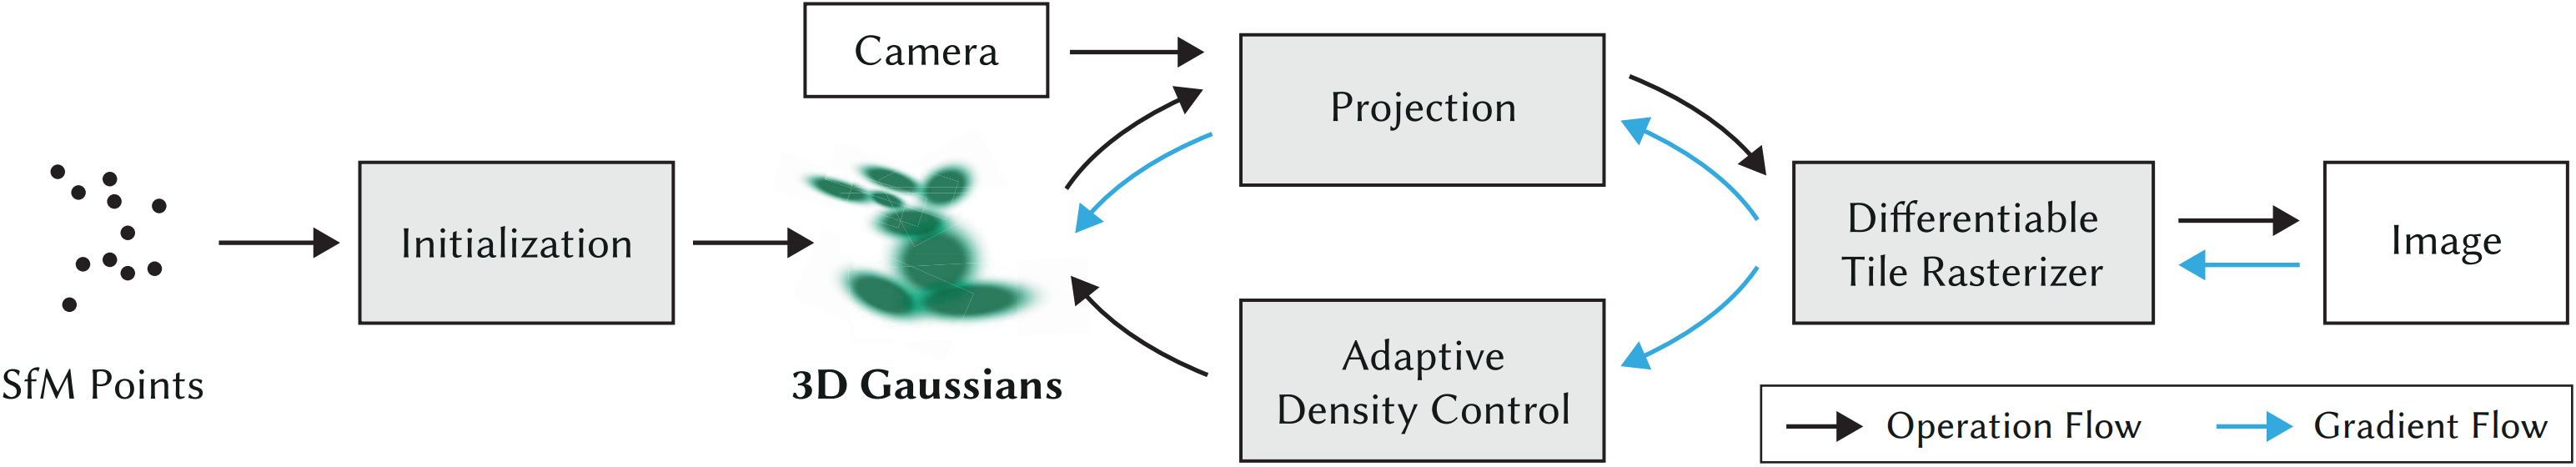
\includegraphics[width=\linewidth]{3dgs-overview.png}
		\caption{Overview of 3DGS}
	\end{figure}
\end{frame}
\begin{frame}[c]
    \Frametitle{Adaptive Density Control}
	\begin{figure}[htbp]
		\centering
		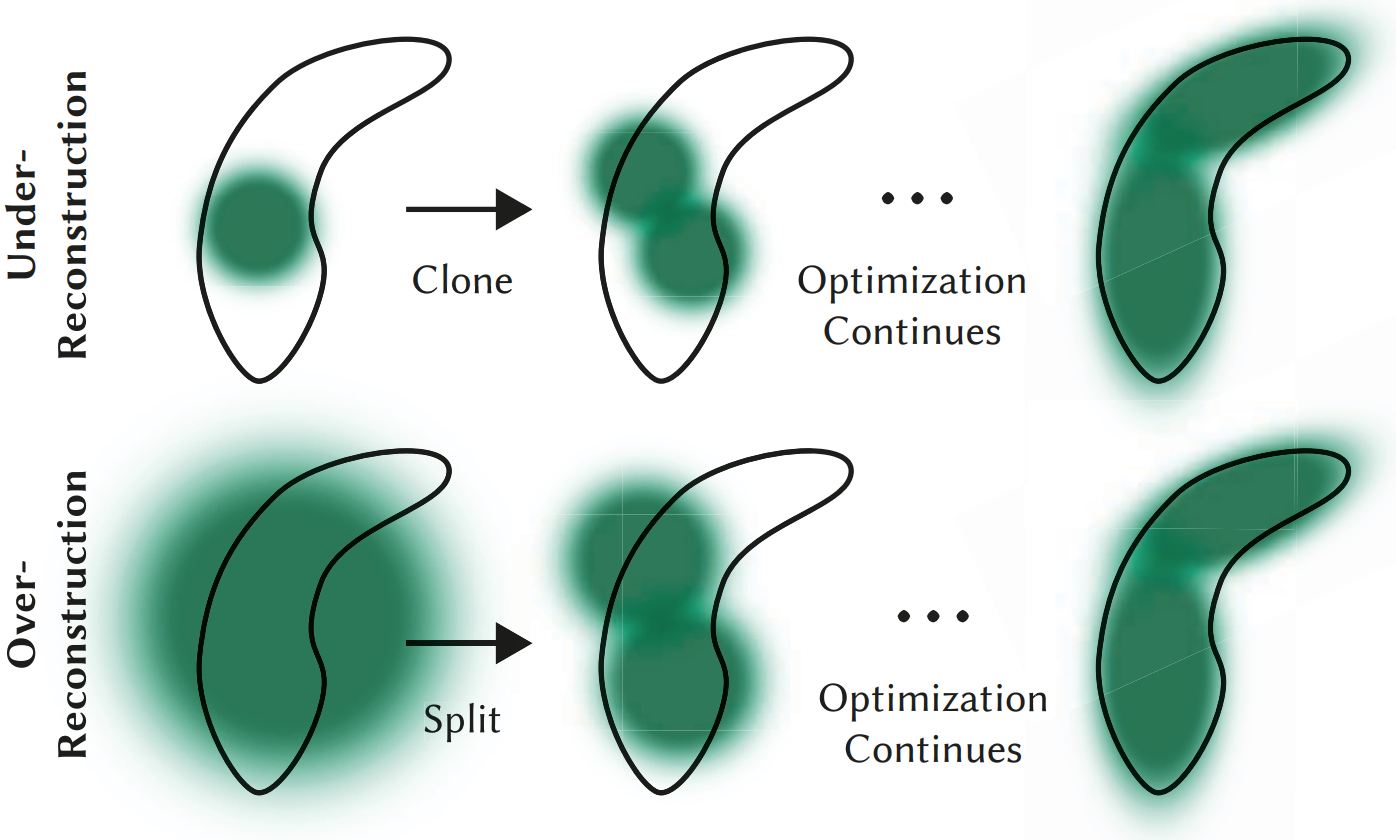
\includegraphics[width=0.5\linewidth]{3dgs-adaptive-densification.png}
		\caption{Adaptive Density Control}
	\end{figure}
\end{frame}


%!Tex Root=**/main.tex

\mode<article>{\chapter{3DGS SLAM}}
\mode<presentation>{\section{3DGS SLAM}}

\mode<article>{\section{Overview}}
\mode<presentation>{\subsection{Overview}}

\begin{frame}\Frametitle{Research Background}
	\colorlet{accepted}{ForestGreen}
	\mode<article>{\par Figure~\ref{fig:3dgs-slam-timeline} shows the timeline of 3DGS SLAM research.}
	\begin{figure}[htbp]
		\centering
		\begin{tikzpicture}
			\usetikzlibrary{calc}
			\usetikzlibrary{positioning}

			\pgfmathsetmacro{\dy}{0.3cm/1pt};
			\pgfmathsetmacro{\nodeNum}{3};
			\pgfmathsetmacro{\sepNum}{\nodeNum-1};
			\pgfmathsetmacro{\length}{0.8*\linewidth};
			\pgfmathsetmacro{\edgeLength}{1cm/1pt};
			\pgfmathsetmacro{\dx}{(\length-\edgeLength-\edgeLength)/\sepNum};
			\pgfmathsetmacro{\xShift}{0};

			\mode<article>{\tikzset{
					node distance=1.5ex,
					note/.style={ anchor=north, align=center, text width=\dx, yshift=-\dy/3, font={\small\sffamily} },
					time/.style={ anchor=south, font={\small\sffamily} },
				}}

			\mode<presentation>{\tikzset{
					node distance=1.5ex,
					note/.style={ anchor=north, align=center, text width=\dx, yshift=-\dy/3, font={\scriptsize\sffamily} },
					time/.style={ anchor=south, font={\scriptsize\sffamily} },
				}}

			\coordinate (start) at (0 pt,0 pt);
			\coordinate (end) at (\length pt,0 pt);
			\draw [line width=1.5pt,-stealth] (start) -- (end);

			\foreach \counter in {0,...,\sepNum} {
					\coordinate (s\counter) at (\edgeLength+\counter*\dx pt,0);
					\coordinate (t\counter) at ($(s\counter)+(0,\dy pt)$);
					\draw [line width=1.5pt] (s\counter) -- (t\counter);
				}

			\node [time] at (t0.north) { 11/2023 - 12/2024 };
			\node [note, below of= s0] (s0_1) { \textcolor{accepted}{SplaTAM}~\autocite{keetha_splatam_2024} };
			\node [note, below of= s0_1] (s0_2) { \textcolor{accepted}{GS-SLAM}~\autocite{yan_gs-slam_2023} };
			\node [note, below of= s0_2] (s0_3) { Gaussian-SLAM~\autocite{yugay_gaussian-slam_2024} };
			\node [note, below of= s0_3] (s0_4) {\textcolor{accepted}{MonoGS}~\autocite{matsuki_gaussian_2024}};
			\node [time] at (t1.north) { 01/2024 - 04/2024 };
			\node [note, below of=s1] (s1_1) {\textcolor{accepted}{RTG-SLAM}~\autocite{peng_rtg-slam_2024}};
			\node [time] at (t2.north) { 05/2024 - 06/2024 };
		\end{tikzpicture}
		\vspace*{0.5ex}
		\caption[Timeline of 3DGS SLAM research]{Timeline of 3DGS SLAM research (\textcolor{accepted}{accepted})}
		\label{fig:3dgs-slam-timeline}
	\end{figure}
\end{frame}

%!Tex Root=**/main.tex
\mode<presentation>{\subsection{Feature-3DGS}}
\mode<article>{\section{Feature-3DGS}}
\begin{frame}
	\Frametitle{Overview}
	\mode<presentation>{\blfootnote{\href{http://arxiv.org/abs/2312.03203}{(CVPR Highlight, 2024) Feature 3DGS: Supercharging 3D Gaussian Splatting to Enable Distilled Feature Fields}}}
	\mode<article>{Figure~\ref{fig:feature-3DGS-overview} is the tagged framework figure of Feature 3DGS~\autocite{zhouFeature3DGSSupercharging2024apr}.}
	\begin{figure}[htbp]
		\begin{annotatedFigureEnv}
			{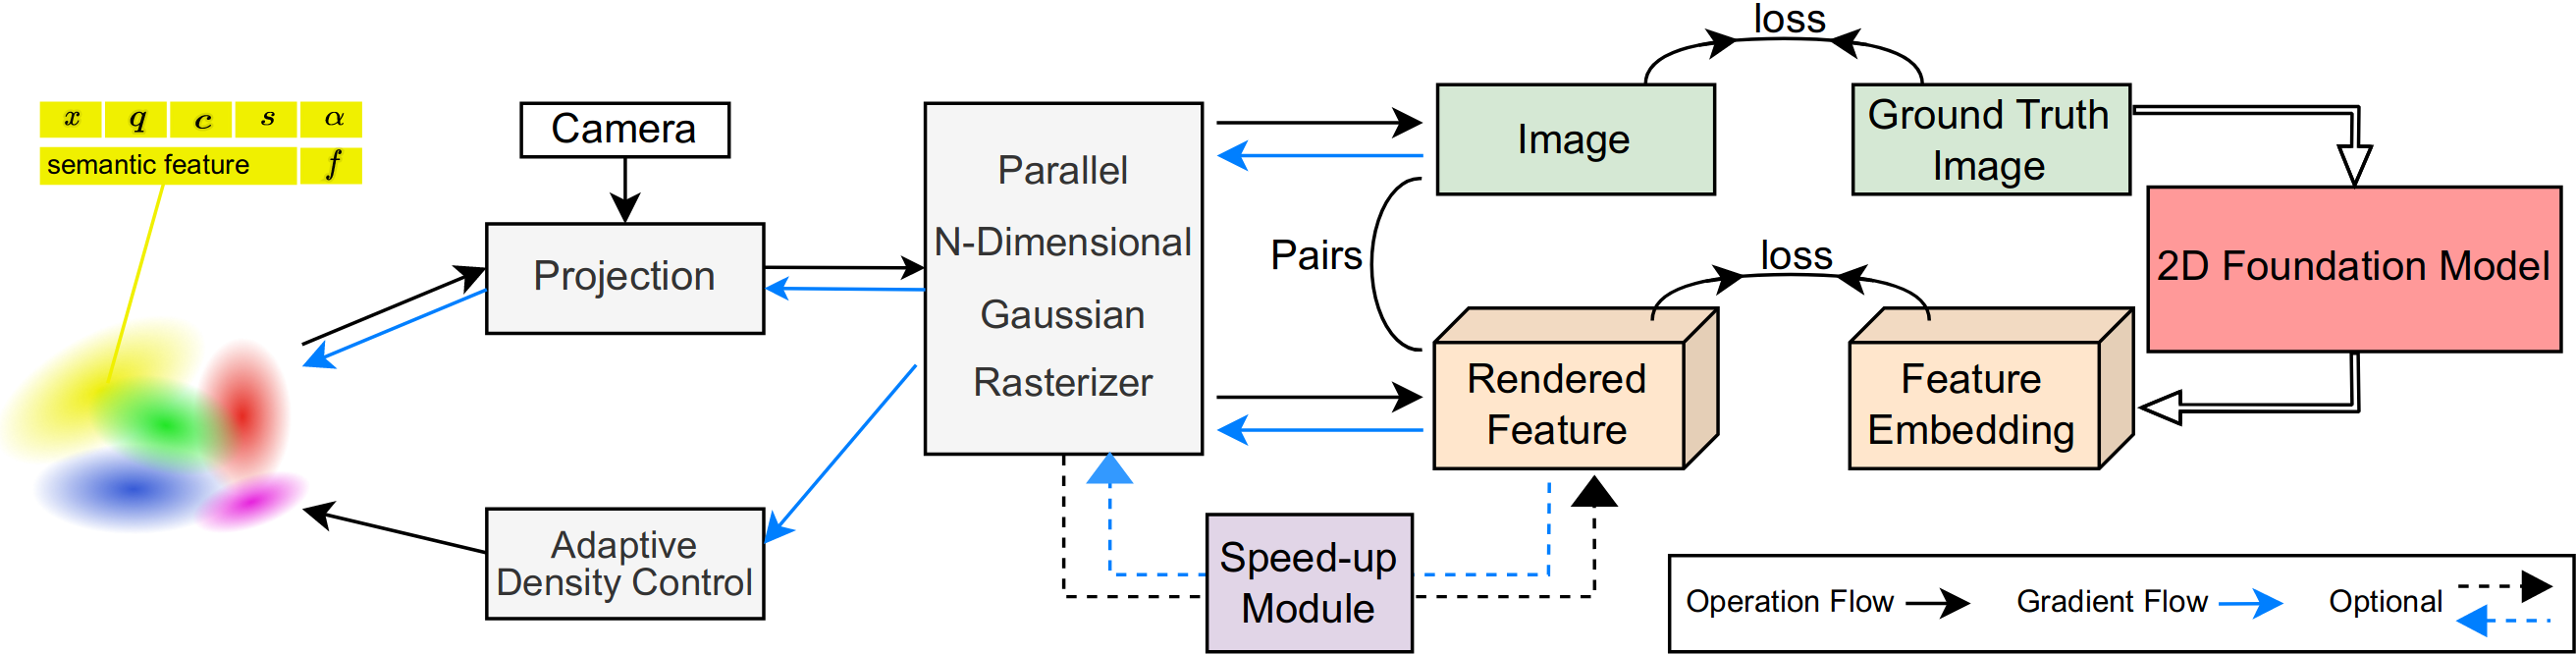
\includegraphics[width=0.85\linewidth]{feature-3dgs-overview.png}}
			\only<1|handout:1>{\annotatedFigure{0,0.7}{0.15,0.78}{1}{0,0.74}}
			\only<1|handout:1>{\annotatedFigure{0.55,0.25}{1,0.72}{1}{0.55,0.72}}
			\only<2->{\annotatedFigure{0.45,-0.05}{0.57,0.25}{2}{0.45,0.25}}
		\end{annotatedFigureEnv}
		\vspace*{0.5ex}
        \caption{Overview of Feature 3DGS~\autocite{zhouFeature3DGSSupercharging2024apr}}
		\label{fig:feature-3DGS-overview}
	\end{figure}
	\mode<presentation>{\vspace*{\fill}}
	\begin{block}{Key Insights}
		\begin{enumerate}
			\mode<presentation>{\setlength{\itemsep}{1.5ex}}
			\item<1-> \alert<1>{Semantic Rendering Pipeline}
				\mode<presentation>{\vspace*{1.5ex}}
				\par Differentiable rendering of Gaussian-wise latent semantic features.
			\item<2-> \alert<2>{Speed-up module}
				\mode<presentation>{\vspace*{1.5ex}}
				\par Dimensionality Alignment.
		\end{enumerate}
	\end{block}
\end{frame}

\begin{frame}\Frametitle{Semantic Rendering Pipeline}
	\mode<presentation>{\blfootnote{\href{http://arxiv.org/abs/2312.03203}{(CVPR Highlight, 2024) Feature 3DGS: Supercharging 3D Gaussian Splatting to Enable Distilled Feature Fields}}}
	\par To render semantic embeddings, i.e. \mode<article>{equation~\ref{eq:feature-3dgs-semantic-rendering}, we have 5 notable things.}
	\begin{figure}[htbp]
		\centering
		\vspace*{2em}
		\resetcolorseries[4]{marknode-color-series}
		\resetcolorseries[4]{annotation-color-series}
		\begin{equation}\label{eq:feature-3dgs-semantic-rendering}
			\mathbb{R}^{
			\alt<3->{\tikzmarknode{n1}{\colorbox{marknode-color-series!![1]}{\scriptsize \(D\)}}}{D}
			}
			\times
			\left\{0,1,\cdots,
			\alt<2->{\tikzmarknode{n0}{\colorbox{marknode-color-series!![0]}{\(N\)}}}{N}
			\right\}
			\times
			\alt<4->{\tikzmarknode{n2}{\colorbox{marknode-color-series!![2]}{\(\left\{\mathcal{F}\right\}\)}}}{\left\{\mathcal{F}\right\}}
			\mapsto
			\left\{0,1,\cdots,
			\alt<5->{\tikzmarknode{n3}{\colorbox{marknode-color-series!![3]}{\(H\)}}}{H}
			\right\}
			\times
			\left\{0,1,\cdots,
			\alt<6->{\tikzmarknode{n4}{\colorbox{marknode-color-series!![4]}{\(W\)}}}{W}
			\right\}
			\times
			\mathbb{R}^{D}
		\end{equation}
		\begin{annotatedEquationEnv}
			\only<2->{\annotatedEquation{colorseries}{n0}{north}{0em}{0.5em}{south west}{annotation-color-series}{number of 3D Gaussians}{east}}
			\only<3->{\annotatedEquation{colorseries}{n1}{north}{0em}{2em}{south west}{annotation-color-series}{dimension of semantic embedding}{east}}
			\only<4->{\annotatedEquation{colorseries}{n2}{south}{0em}{-0.5em}{north east}{annotation-color-series}{camera frames}{west}}
			\only<5->{\annotatedEquation{colorseries}{n3}{south}{0em}{-0.5em}{north east}{annotation-color-series}{image height}{west}}
			\only<6->{\annotatedEquation{colorseries}{n4}{south}{0em}{-0.5em}{north east}{annotation-color-series}{image width}{west}}
		\end{annotatedEquationEnv}
		\vspace*{0.5em}
	\end{figure}
	\mode<presentation>{
		\mode<presentation>{\vspace*{\fill}}
		\begin{minipage}[c]{0.35\linewidth}
			\definecolor{feature-3dgs-blue}{HTML}{007FFF}
			\uncover<7->{\par 5 things,}
			\mode<presentation>{\vspace*{1.5ex}}
			\begin{enumerate}[<+(7)- |alert@.(8)>]
				\mode<presentation>{\setlength{\itemsep}{1.5ex}}
				\item representation
				\item projection
				\item blending
				\item rasterization
				\item \textcolor{feature-3dgs-blue}{inverse rendering}
			\end{enumerate}
		\end{minipage}
		\mode<presentation>{\begin{minipage}[c]{0.60\linewidth}
				\centering
				\begin{uncoverenv}<7->
					\adjustbox{trim={.01\width} {.01\height} {.5\width} {.1\height}, clip}{
						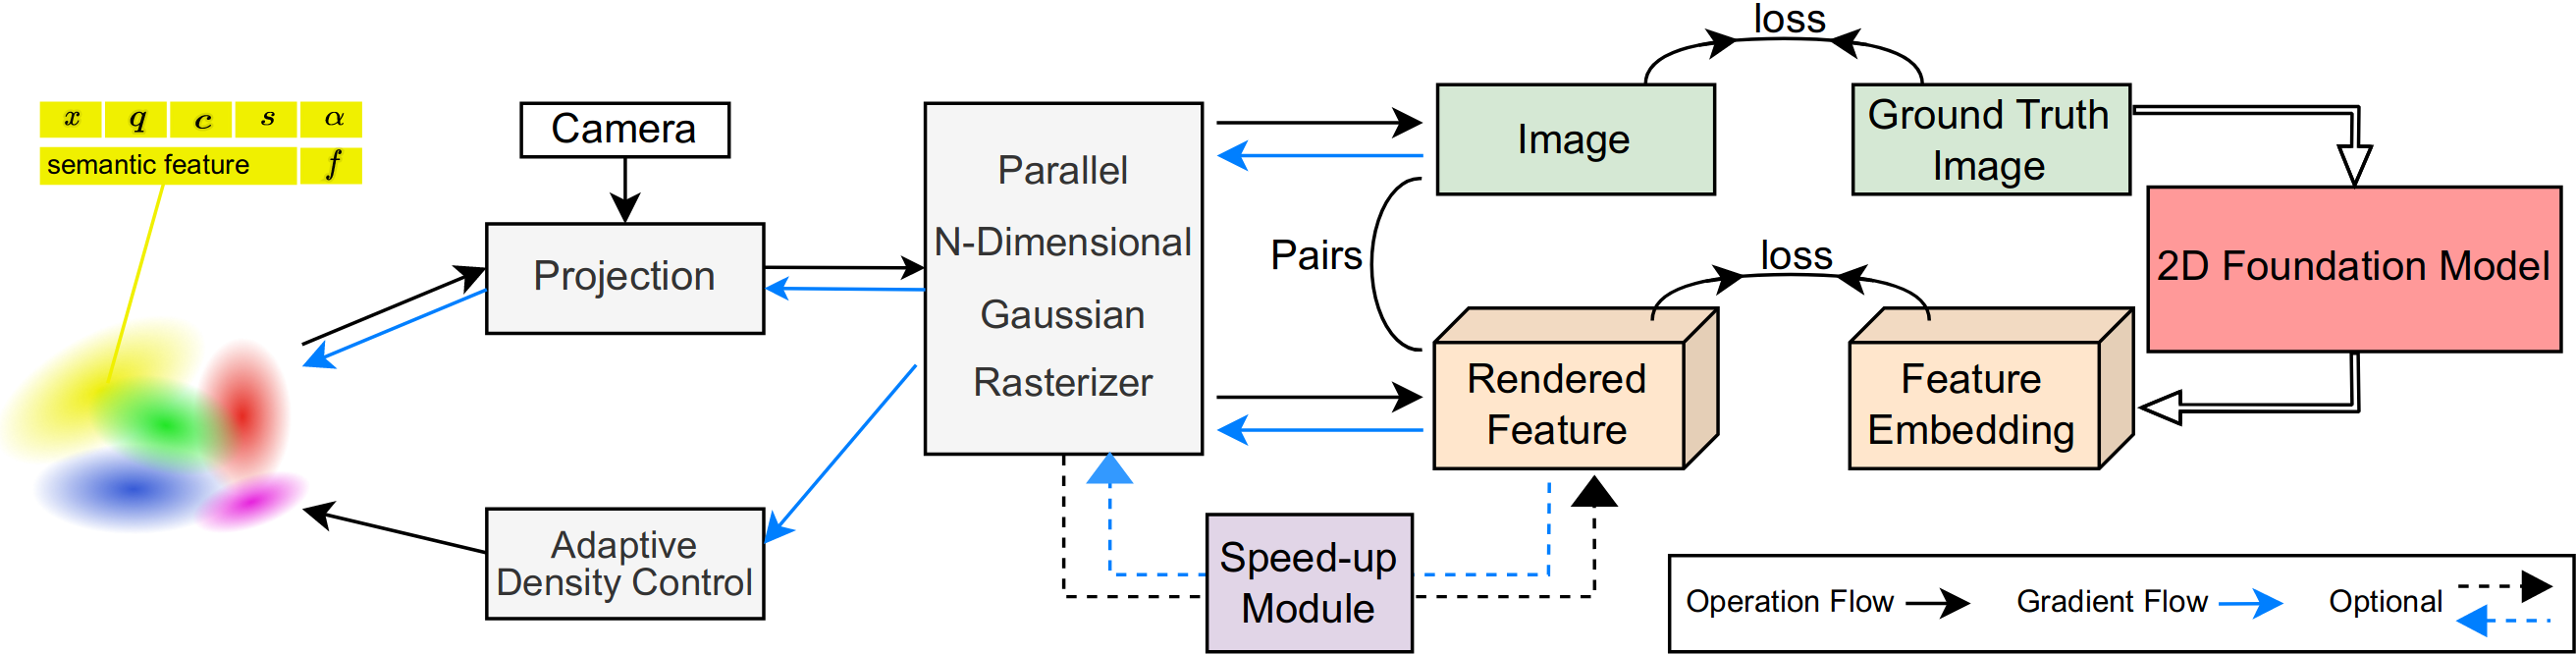
\includegraphics[width=1.5\linewidth]{feature-3dgs-overview.png}
					}
				\end{uncoverenv}
			\end{minipage}}
	}
\end{frame}

\begin{frame}\mode<presentation>{\Frametitle{Semantic Rendering Pipeline \romannum{1}}}
	\mode<presentation>{\blfootnote{\href{http://arxiv.org/abs/2312.03203}{(CVPR Highlight, 2024) Feature 3DGS: Supercharging 3D Gaussian Splatting to Enable Distilled Feature Fields}}}
	\begin{block}{Representation\hfill Semantic Rendering Pipeline \romannum{1}}
		\par \alert<+>{Representation}: 3D Gaussian augmented with a latent embedding.
        \footnote{For color representation, \(n\) is the maximal order of spherical harmonics for a color channel. \(n=4\) in practice.}
        \mode<article>{(equation~\ref{eq:feature-3dgs-semantic-gaussian})}
		\resetcolorseries[8]{marknode-color-series}
		\resetcolorseries[8]{annotation-color-series}
		\begin{equation}\label{eq:feature-3dgs-semantic-gaussian}
			\alt<2-|handout:1>{\tikzmarknode{n0}{\colorbox{marknode-color-series!![0]}{\(\mathcal{G}\)}}}{\mathcal{G}}
			_{
			\alt<3-|handout:1>{\tikzmarknode{n1}{\colorbox{marknode-color-series!![1]}{\scriptsize \(i\)}}}{i}
			}
			=
			\left\{
			\alt<4-|handout:1>{\tikzmarknode{n2}{\colorbox{marknode-color-series!![2]}{\(\mathbf{x}\)},}}{\mathbf{x},}
			\alt<5-|handout:1>{\tikzmarknode{n3}{\colorbox{marknode-color-series!![3]}{\(\mathbf{q}\)},}}{\mathbf{q},}
			\alt<6-|handout:1>{\tikzmarknode{n4}{\colorbox{marknode-color-series!![4]}{\(\mathbf{s}\)},}}{\mathbf{s},}
			\alt<7-|handout:1>{\tikzmarknode{n5}{\colorbox{marknode-color-series!![5]}{\(\alpha\)},}}{\alpha,}
			\alt<8-|handout:1>{\tikzmarknode{n6}{\colorbox{marknode-color-series!![6]}{\(\mathbf{c}\)},}}{\mathbf{c},}
			\alt<9-|handout:1>{\tikzmarknode{n7}{\colorbox{marknode-color-series!![7]}{\(\mathbf{f}\)},}}{\mathbf{f}}
			\right\}
		\end{equation}
		\begin{annotatedEquationEnv}
			\only<2-|handout:1>{\annotatedEquation{colorseries}{n0}{south}{0em}{-0.5em}{north east}{annotation-color-series}{optimizable 3D Gaussian}{west}}
			\only<3-|handout:1>{\annotatedEquation{colorseries}{n1}{south}{0em}{-2em}{north east}{annotation-color-series}{\(\in \mathbb{N}\), index of 3D Gaussian}{west}}
			\only<4-|handout:1>{\annotatedEquation{colorseries}{n2}{south}{0em}{-8em}{north west}{annotation-color-series}{\(\in \mathbb{R}^{3}\), position}{east}}
			\only<5-|handout:1>{\annotatedEquation{colorseries}{n3}{south}{0em}{-6.5em}{north west}{annotation-color-series}{\(\in \mathrm{SO}(3)\), rotation}{east}}
			\only<6-|handout:1>{\annotatedEquation{colorseries}{n4}{south}{0em}{-5em}{north west}{annotation-color-series}{\(\in \mathbb{R}^{3}\), scale}{east}}
			\only<7-|handout:1>{\annotatedEquation{colorseries}{n5}{south}{0em}{-3.5em}{north west}{annotation-color-series}{\(\in [0,1]\), opacity}{east}}
			\only<8-|handout:1>{\annotatedEquation{colorseries}{n6}{south}{0em}{-2em}{north west}{annotation-color-series}{\(\in \mathbb{R}^{3n}\), color}{east}}
			\only<9-|handout:1>{\annotatedEquation{colorseries}{n7}{south}{0em}{-0.5em}{north west}{annotation-color-series}{\(\boldmath \in \mathbb{R}^{3}\), semantic feature}{east}}
		\end{annotatedEquationEnv}
		\vspace*{8em}
	\end{block}
\end{frame}

\begin{frame}
	\mode<presentation>{\Frametitle{Semantic Rendering Pipeline \romannum{2}}}

	\mode<presentation>{\blfootnote{\href{http://arxiv.org/abs/2312.03203}{(CVPR Highlight, 2024) Feature 3DGS: Supercharging 3D Gaussian Splatting to Enable Distilled Feature Fields}}}

	\begin{block}{Projection\hfill Semantic Rendering Pipeline \romannum{2}}
		\par \alert<.>{Projection}: from 3D ellipsoids to 2D ellipses. \mode<article>{(equation~\ref{eq:feature-3dgs-projection-mean} and~\ref{eq:feature-3dgs-projection-covariance})}
		\begin{minipage}[t]{0.45\linewidth}
			\resetcolorseries[4]{marknode-color-series}
			\resetcolorseries[4]{annotation-color-series}
			\begin{align}\label{eq:feature-3dgs-projection-mean}
				\alt<5->{\tikzmarknode{n3}{\colorbox{marknode-color-series!![3]}{\(\mu_{i}\)}}}{\mu_{i}}
				=
				\alt<4->{\tikzmarknode{n2}{\colorbox{marknode-color-series!![2]}{\(\pi\)}}}{\pi}
				\left(
				\alt<3->{\tikzmarknode{n1}{\colorbox{marknode-color-series!![1]}{\(\mathbf{T}_{cw}\)}}}{\mathbf{T}_{cw}}
				\cdot
				\alt<2->{\tikzmarknode{n0}{\colorbox{marknode-color-series!![0]}{\(\mu_{w}\)}}}{\mu_{w}}
				\right)
			\end{align}
			\begin{annotatedEquationEnv}
				\only<2->{\annotatedEquation{colorseries}{n0}{south}{0em}{-1em}{north west}{annotation-color-series}{\(\in \mathbb{P}^3\), 3D(world) mean}{east}}
				\only<3->{\annotatedEquation{colorseries}{n1}{south}{0em}{-3em}{north west}{annotation-color-series}{\(\in \mathrm{SE}(3)\), camera pose}{east}}
				\only<4->{\annotatedEquation{colorseries}{n2}{south}{0em}{-5em}{north west}{annotation-color-series}{projection}{east}}
				\only<5->{\annotatedEquation{colorseries}{n3}{south}{0}{-7em}{north west}{annotation-color-series}{\(\in \mathbb{P}^2\), 2D(image) mean}{east}}
			\end{annotatedEquationEnv}
		\end{minipage}
		\hspace*{\fill}
		\begin{minipage}[t]{0.50\linewidth}
			\resetcolorseries[4]{marknode-color-series}
			\resetcolorseries[4]{annotation-color-series}
			\begin{align}\label{eq:feature-3dgs-projection-covariance}
				\alt<9->{\tikzmarknode{n3}{\colorbox{marknode-color-series!![3]}{\(\Sigma_{i}\)}}}{\Sigma_{i}}
				=
				\alt<8->{\tikzmarknode{n2}{\colorbox{marknode-color-series!![2]}{\(\mathbf{J}_{\pi}\)}}}{\mathbf{J}_{\pi}}
				\alt<7->{\tikzmarknode{n1}{\colorbox{marknode-color-series!![1]}{\(\mathbf{R}_{cw}\)}}}{\mathbf{R}_{cw}}
				\alt<6->{\tikzmarknode{n0}{\colorbox{marknode-color-series!![0]}{\(\Sigma_{w}\)}}}{\Sigma_{w}}  \mathbf{R}_{cw}^{\mathrm{T}} \mathbf{J}_{\pi}^{\mathrm{T}}
			\end{align}
			\begin{annotatedEquationEnv}
				\only<6->{\annotatedEquation{colorseries}{n0}{south}{0em}{-1em}{north west}{annotation-color-series}{\(\in \mathbb{R}^{3\times 3}\),\\3D(world) covariance}{east}}
				\only<7->{\annotatedEquation{colorseries}{n1}{south}{0em}{-3.5em}{north west}{annotation-color-series}{\(\in \mathrm{SO(3)}\),\\rotation component of \(\mathbf{T}_{cw}\)}{east}}
				\only<8->{\annotatedEquation{colorseries}{n2}{south}{0em}{-6em}{north west}{annotation-color-series}{\(\in \mathbb{R}^{2\times 3}\), Jacobian of the \\linear approximation of \(\pi\)}{east}}
				\only<9->{\annotatedEquation{colorseries}{n3}{south}{0em}{-8.5em}{north west}{annotation-color-series}{\(\in \mathbb{R}^{2\times 2}\), 2D(image) covariance}{east}}
			\end{annotatedEquationEnv}
		\end{minipage}
		\vspace*{8.5em}
	\end{block}
\end{frame}
% 
\begin{frame}
	\mode<presentation>{\Frametitle{Semantic Rendering Pipeline \romannum{3}}}

	\mode<presentation>{\blfootnote{\href{http://arxiv.org/abs/2312.03203}{(CVPR Highlight, 2024) Feature 3DGS: Supercharging 3D Gaussian Splatting to Enable Distilled Feature Fields}}}
	\begin{block}{Blending\hfill Semantic Rendering Pipeline \romannum{3}}
		\par \alert{Blending}: $\alpha$-blending of semantic embeddings. \mode<article>{(equation~\ref{eq:feature-3dgs-semantic-alpha-blending})}
		\vspace*{1em}
		\resetcolorseries[5]{marknode-color-series}
		\resetcolorseries[5]{annotation-color-series}
		\begin{equation}\label{eq:feature-3dgs-semantic-alpha-blending}
			\alt<2->{\tikzmarknode{n0}{\colorbox{marknode-color-series!![0]}{\(\mathbf{f}(h,w)\)}}}{\mathbf{f}(h,w)}
			=
			\sum_{i=1}^{
			\alt<6->{\tikzmarknode{n4}{\colorbox{marknode-color-series!![4]}{\scriptsize \(N\)}}}{N}
			}
			\alt<5->{\tikzmarknode{n3}{\colorbox{marknode-color-series!![3]}{\(T_i\)}}}{T_i}
			\alt<4->{\tikzmarknode{n2}{\colorbox{marknode-color-series!![2]}{\(\alpha_i\)}}}{\alpha_i}
			\alt<3->{\tikzmarknode{n1}{\colorbox{marknode-color-series!![1]}{\(\mathbf{f}_i(h,w)\)}}}{\mathbf{f}_i(h,w)}
			,\quad
			\uncover<5->{T_i = \prod_{j=1}^{i-1} (1-\alpha_j)}
		\end{equation}
		\begin{annotatedEquationEnv}
			\only<2->{\annotatedEquation{colorseries}{n0}{south}{0em}{-0.5em}{north east}{annotation-color-series}{semantic feature\\on pixel \((h,w)\)}{west}}
			\only<3->{\annotatedEquation{colorseries}{n1}{south}{0em}{-1em}{north west}{annotation-color-series}{semantic feature of \(i\)-th Gaussian on pixel \((h,w)\)}{east}}
			\only<4->{\annotatedEquation{colorseries}{n2}{south}{0em}{-2.5em}{north west}{annotation-color-series}{opacity of \(i\)-th Gaussian}{east}}
			\only<5->{\annotatedEquation{colorseries}{n3}{south}{0em}{-4em}{north west}{annotation-color-series}{background opacity for \(i\)-th Gaussian}{east}}
			\only<6->{\annotatedEquation{colorseries}{n4}{north}{0em}{0.5em}{south west}{annotation-color-series}{number of the \textbf{sorted \& visible} subset of 3D Gaussians}{east}}
		\end{annotatedEquationEnv}
		\vspace*{4em}
	\end{block}
\end{frame}

\begin{frame}
	\mode<presentation>{\Frametitle{Semantic Rendering Pipeline \romannum{4}}}

	\mode<presentation>{\blfootnote{\href{http://arxiv.org/abs/2312.03203}{(CVPR Highlight, 2024) Feature 3DGS: Supercharging 3D Gaussian Splatting to Enable Distilled Feature Fields}}}

	\mode<presentation>{
		\vspace*{1.5ex}
		\begin{minipage}[c]{0.25\linewidth}
			\centering
			\adjustbox{trim={.30\width} {.30\height} {.50\width} {.01\height}, clip}{
				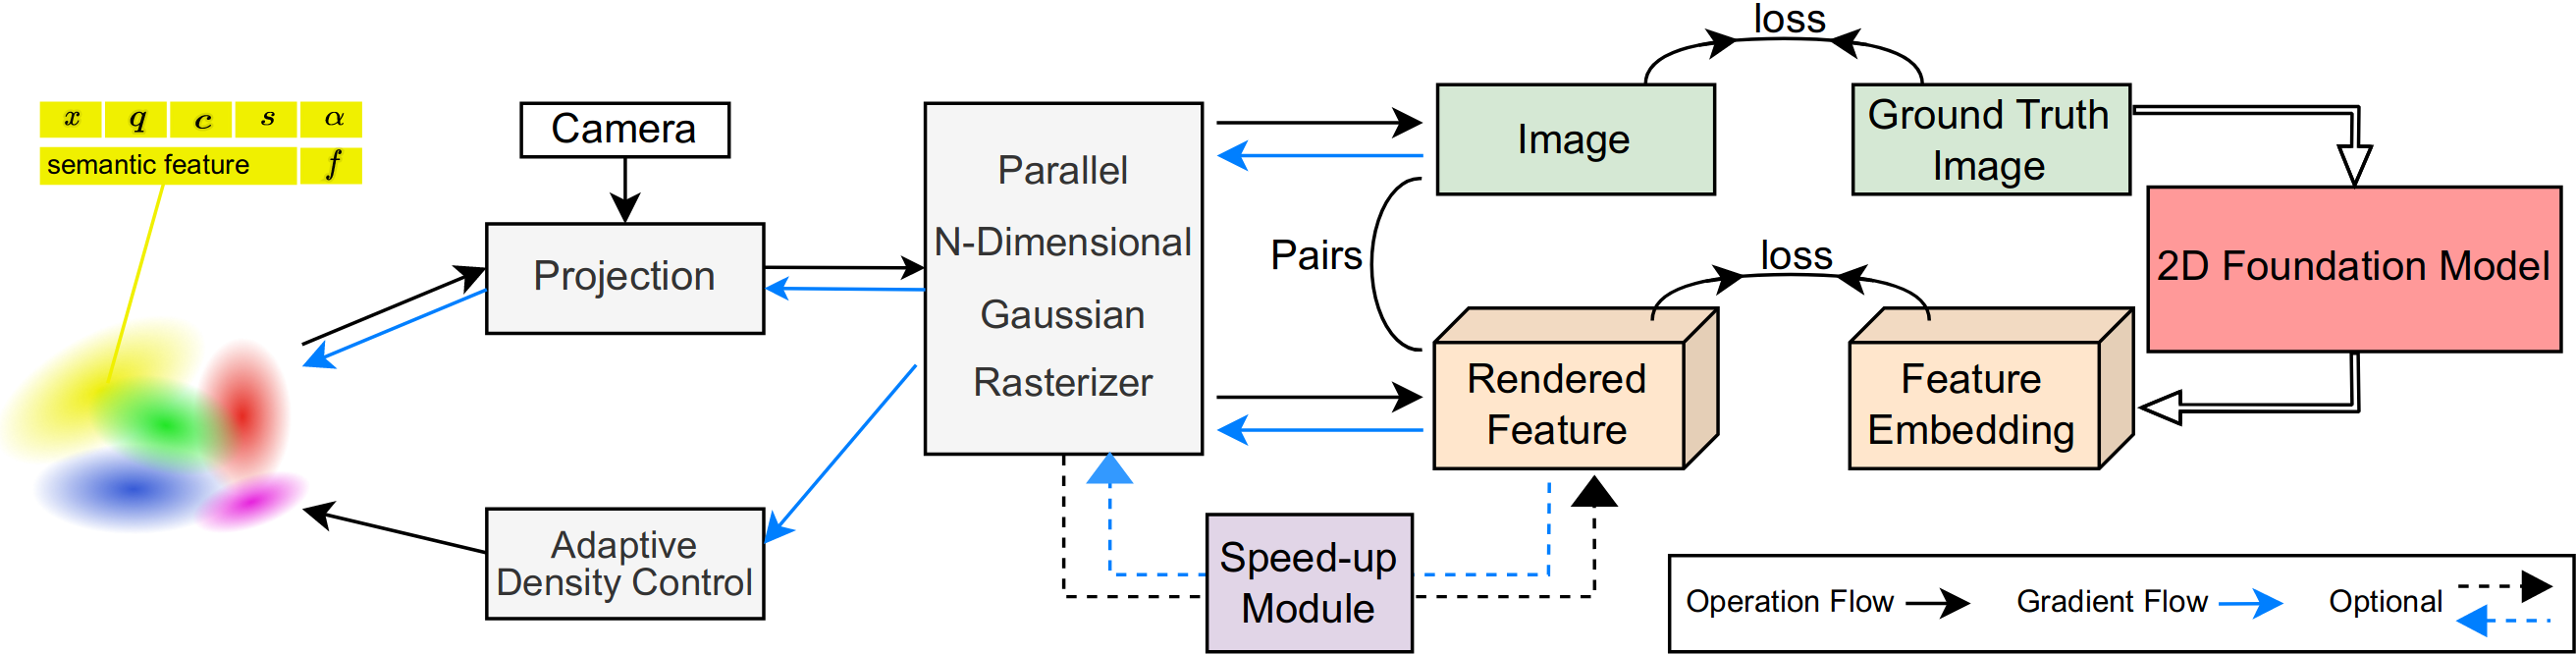
\includegraphics[width=4\linewidth]{feature-3dgs-overview.png}
			}
		\end{minipage}
		\hspace{\fill}
	}

	\begin{block}{Rasterization\hfill Semantic Rendering Pipeline \romannum{4}}
		\par \alert{Rasterization}: tiled and implemented in CUDA.
		\begin{itemize}[<+(1)->]
			\mode<presentation>{\setlength{\itemsep}{1.5ex}}
			\item \alert<.(1)|handout:0>{Divide} the screen space into tiles (CUDA thread blocks).
			\item \alert<.(1)|handout:0>{Group} the Gaussians by view frustum and tile index.
			\item \alert<.(1)|handout:0>{Sort} the Gaussians by front-to-back depth order.
			\item \alert<.(1)|handout:0>{Blend} each pixel within a tile in parallel (CUDA threads).
		\end{itemize}
	\end{block}
\end{frame}

\begin{frame}
	\mode<presentation>{\Frametitle{Semantic Rendering Pipeline \romannum{5}}}

	\mode<presentation>{\blfootnote{\href{http://arxiv.org/abs/2312.03203}{(CVPR Highlight, 2024) Feature 3DGS: Supercharging 3D Gaussian Splatting to Enable Distilled Feature Fields}}}
	\begin{block}{Inverse Rendering\hfill Semantic Rendering Pipeline \romannum{5}}
		\par \alert<1->{Inverse rendering}: guided by image-wise photometric loss.
		\footnote{\(\gamma=1, \lambda=0.2.\)}
		\mode<article>{(equation \ref{eq:feature-3dgs-loss}, \ref{eq:feature-3dgs-appearance-loss} and \ref{eq:feature-3dgs-semantic-loss})}
		\resetcolorseries[2]{marknode-color-series}
		\resetcolorseries[2]{annotation-color-series}
		\begin{equation}\label{eq:feature-3dgs-loss}
			\mathcal{L} = \mathcal{L}_{appearance} + \gamma \mathcal{L}_{semantics}
		\end{equation}
		\vspace*{1.2em}
		\begin{alignat}{2}
			\label{eq:feature-3dgs-appearance-loss} & \mathcal{L}_{appearance} &  & = (1-\lambda) \mathcal{L}_{1} \left(
			\tikzmarknode{n0}{\colorbox{marknode-color-series!![0]}{\(\mathbf{C}\)}}
			,
			\tikzmarknode{n1}{\colorbox{marknode-color-series!![0]}{\(\hat{\mathbf{C}}\)}}
			\right) + \lambda \mathcal{L}_{D-SSIM}\left(\mathbf{C}, \hat{\mathbf{C}}\right)                              \\
			\label{eq:feature-3dgs-semantic-loss}   & \mathcal{L}_{semantics}  &  & = \mathcal{L}_{1} \left(
			\tikzmarknode{n2}{\colorbox{marknode-color-series!![1]}{\(\mathbf{F}\)}}
			,\tikzmarknode{n3}{\colorbox{marknode-color-series!![1]}{\(\hat{\mathbf{F}}\)}}
			\right) = \sum_{h=1}^{H} \sum_{w=1}^{W} \Vert \mathbf{f}{(h, w)} - \hat{\mathbf{f}}{(h, w)} \Vert_1
		\end{alignat}
		\begin{annotatedEquationEnv}
			\annotatedEquation{color}{n0}{north}{0em}{1.2em}{south east}{annotation-color-series!!}{captured RGB image (ground-truth)}{west}
			\annotatedEquation{color}{n1}{north}{0em}{1em}{south west}{annotation-color-series!!}{rendered RGB image}{east}
			\textcolor{annotation-color-series!!+}{}%
			\annotatedEquation{color}{n2}{south}{0em}{-1.5em}{north east}{annotation-color-series!!}{inferred semantic feature map}{west}
			\annotatedEquation{color}{n3}{south}{0em}{-1.5em}{north west}{annotation-color-series!!}{rendered semantic feature map}{east}
		\end{annotatedEquationEnv}
		\vspace*{1.5em}
	\end{block}
\end{frame}

\begin{frame}
	\Frametitle{Speed-up Module}
	\begin{block}<+->{Motivation}
		\par Too \emph{inefficient} to embed naively,
		\begin{enumerate}[<+->]
			\mode<presentation>{\setlength{\itemsep}{1.5ex}}
			\item \alert<.>{High dimension:} latent features in large foundation models.
			      \footnote{e.g. \(512\) for CLIP; \(256\) for SAM.}
			\item \alert<.>{Large quantities:} millions of Gaussians in a scene.
		\end{enumerate}
	\end{block}
	\mode<presentation>{\vspace*{\fill}}
	\begin{block}<+->{Solution}
		\begin{enumerate}[<+->]
			\mode<presentation>{\setlength{\itemsep}{1.5ex}}
			\item \alert<.>{Compactness:} to embed Gaussians with more compact vectors, \(\dim = D^{\,\prime} < D\).
			\item \alert<.>{Alignment:} to align the dimensionalities using a lightweight decoder.\footnote{Lightweight decoder: In practice, a \(1\times 1\) convolutional layer or a fully-connected layer.}
		\end{enumerate}
	\end{block}
	\mode<presentation>{\blfootnote{\href{http://arxiv.org/abs/2312.03203}{(CVPR Highlight, 2024) Feature 3DGS: Supercharging 3D Gaussian Splatting to Enable Distilled Feature Fields}}}
\end{frame}

\begin{frame}
	\Frametitle{Summary}
	\mode<presentation>{\blfootnote{\href{http://arxiv.org/abs/2312.03203}{(CVPR Highlight, 2024) Feature 3DGS: Supercharging 3D Gaussian Splatting to Enable Distilled Feature Fields}}}
	\begin{block}{Limitations}
		\begin{enumerate}[<+->]
			\mode<presentation>{\setlength{\itemsep}{1.5ex}}
			\item Inefficiency
			      \mode<presentation>{\vspace*{1.5ex}}
			      \begin{itemize}
				      \mode<presentation>{\setlength{\itemsep}{1.5ex}}
				      \item ``Speed-up module'' is not enough,
				            \uncover<+->{
					            \mode<presentation>{\vspace*{1.5ex}}
					            \par \(\dim = 128\) embedding for millions of Gaussians.
				            }
			      \end{itemize}
			      \mode<presentation>{\vspace*{1.5ex}}
			\item 3D Inconsistency \& Inaccuracy
			      \mode<presentation>{\vspace*{1.5ex}}
			      \begin{itemize}
				      \mode<presentation>{\setlength{\itemsep}{1.5ex}}
				      \item 2D foundation models are still 2D.
			      \end{itemize}
		\end{enumerate}
	\end{block}
\end{frame}


%!Tex Root=**/main.tex
\mode<presentation>{\subsection{LangSplat}}
\mode<article>{\section{LangSplat}}

\begin{frame}<article>[c]
	\mode<all>{\Frametitle{Overview}}% Customized Title
    \mode<article>{Figure~\ref{fig:langsplat-overview} is the tagged framework of~\autocite{qinLangSplat3DLanguage2023}.}
	\begin{figure}[htbp]
		\centering
		\begin{annotatedFigureEnv}
			{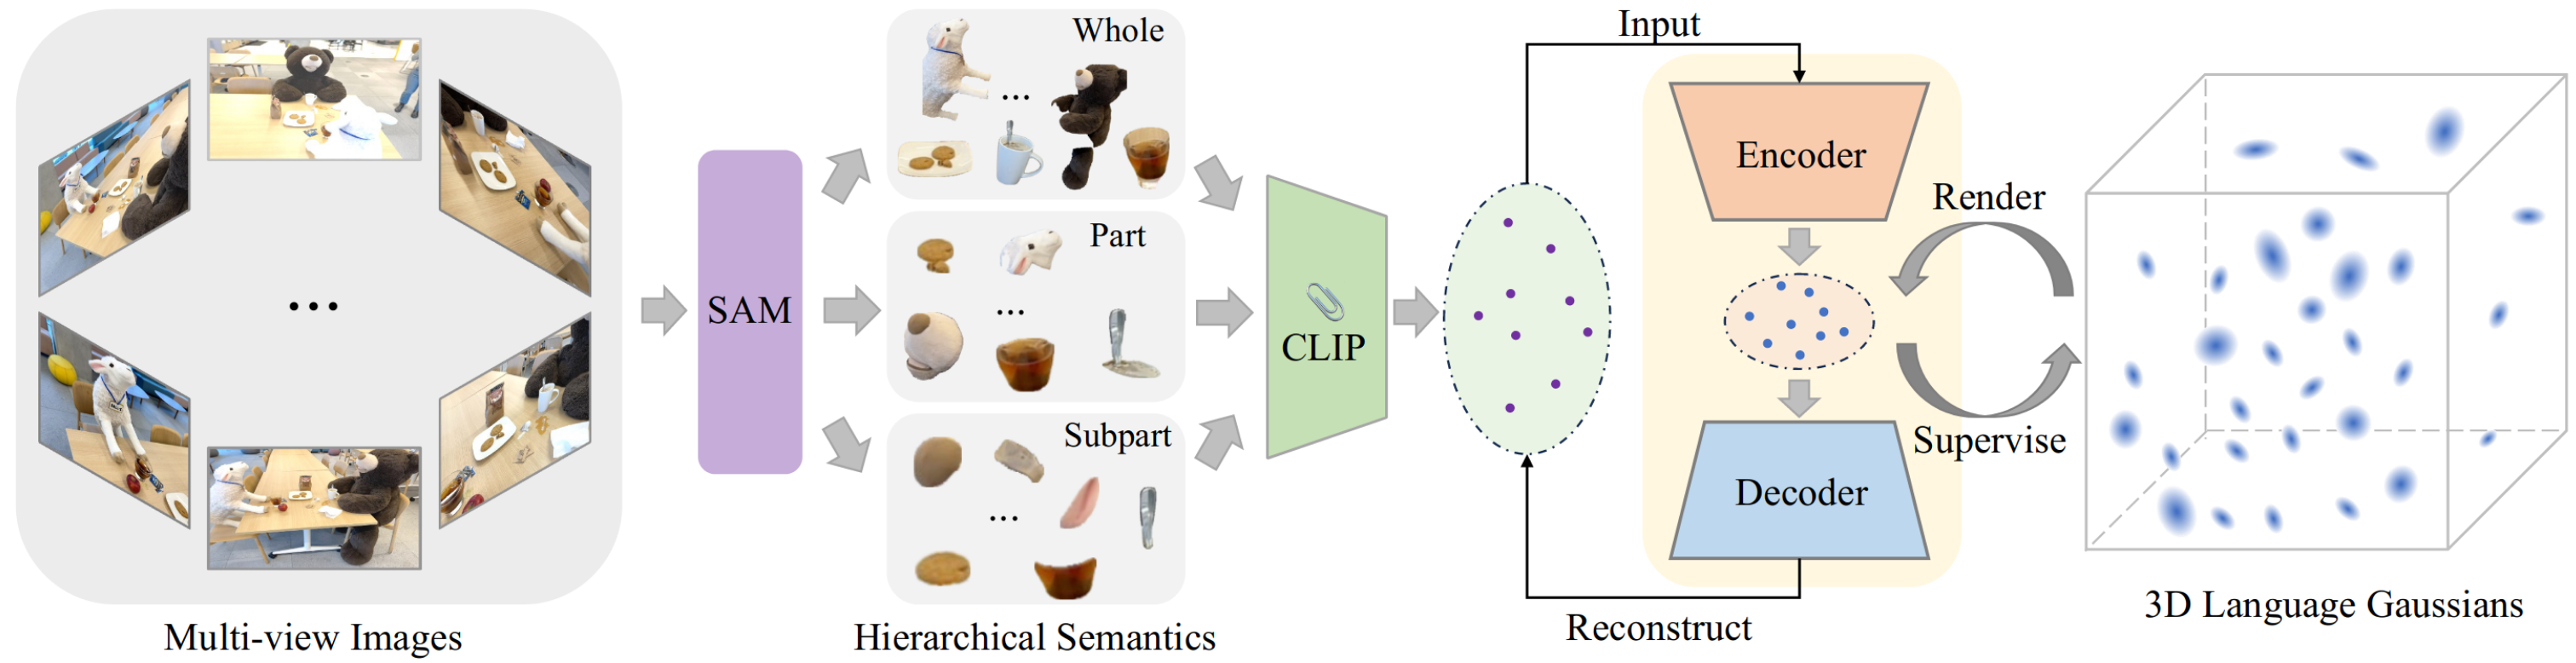
\includegraphics[width=0.8\linewidth]{langsplat-overview.png}}
			\annotatedFigure{0.25,0}{0.55,1}{1}{0.25,0}
			\annotatedFigure{0.55,0}{0.82,1}{2}{0.55,0}
		\end{annotatedFigureEnv}
		\vspace*{0.5ex}
        \caption{Overview of LangSplat~\autocite{qinLangSplat3DLanguage2023}}
        \label{fig:langsplat-overview}
	\end{figure}
	\begin{block}{Key Insights}
		\begin{enumerate}
			\item \alert{Accuracy:} SAM outputs to enhance CLIP features.
			      \begin{itemize}
				      \item \alert{CLIP:} image-aligned training leads to ``point-ambiguity''.
				      \item \alert{SAM:} pixel-aligned \& object-centered \& multi-granularity.
			      \end{itemize}
			\item \alert{Efficiency:} an \alert{auto-encoder} to compress latent features.
			      \begin{itemize}
				      \item More complexity and better compression, compared with ``speed-up module'' in Feature 3DGS~\autocite{zhouFeature3DGSSupercharging2024apr}.
			      \end{itemize}
		\end{enumerate}
	\end{block}
	\mode<presentation>{\blfootnote{\href{http://arxiv.org/abs/2312.16084}{(CVPR Highlight, 2024) LangSplat: 3D Language Gaussian Splatting}}}
\end{frame}

\begin{frame}<presentation>
	\Frametitle{Overview}
	\mode<presentation>{\blfootnote{\href{http://arxiv.org/abs/2312.16084}{(CVPR Highlight, 2024) LangSplat: 3D Language Gaussian Splatting}}}
	\begin{figure}[htbp]
		\centering
		\begin{annotatedFigureEnv}
			{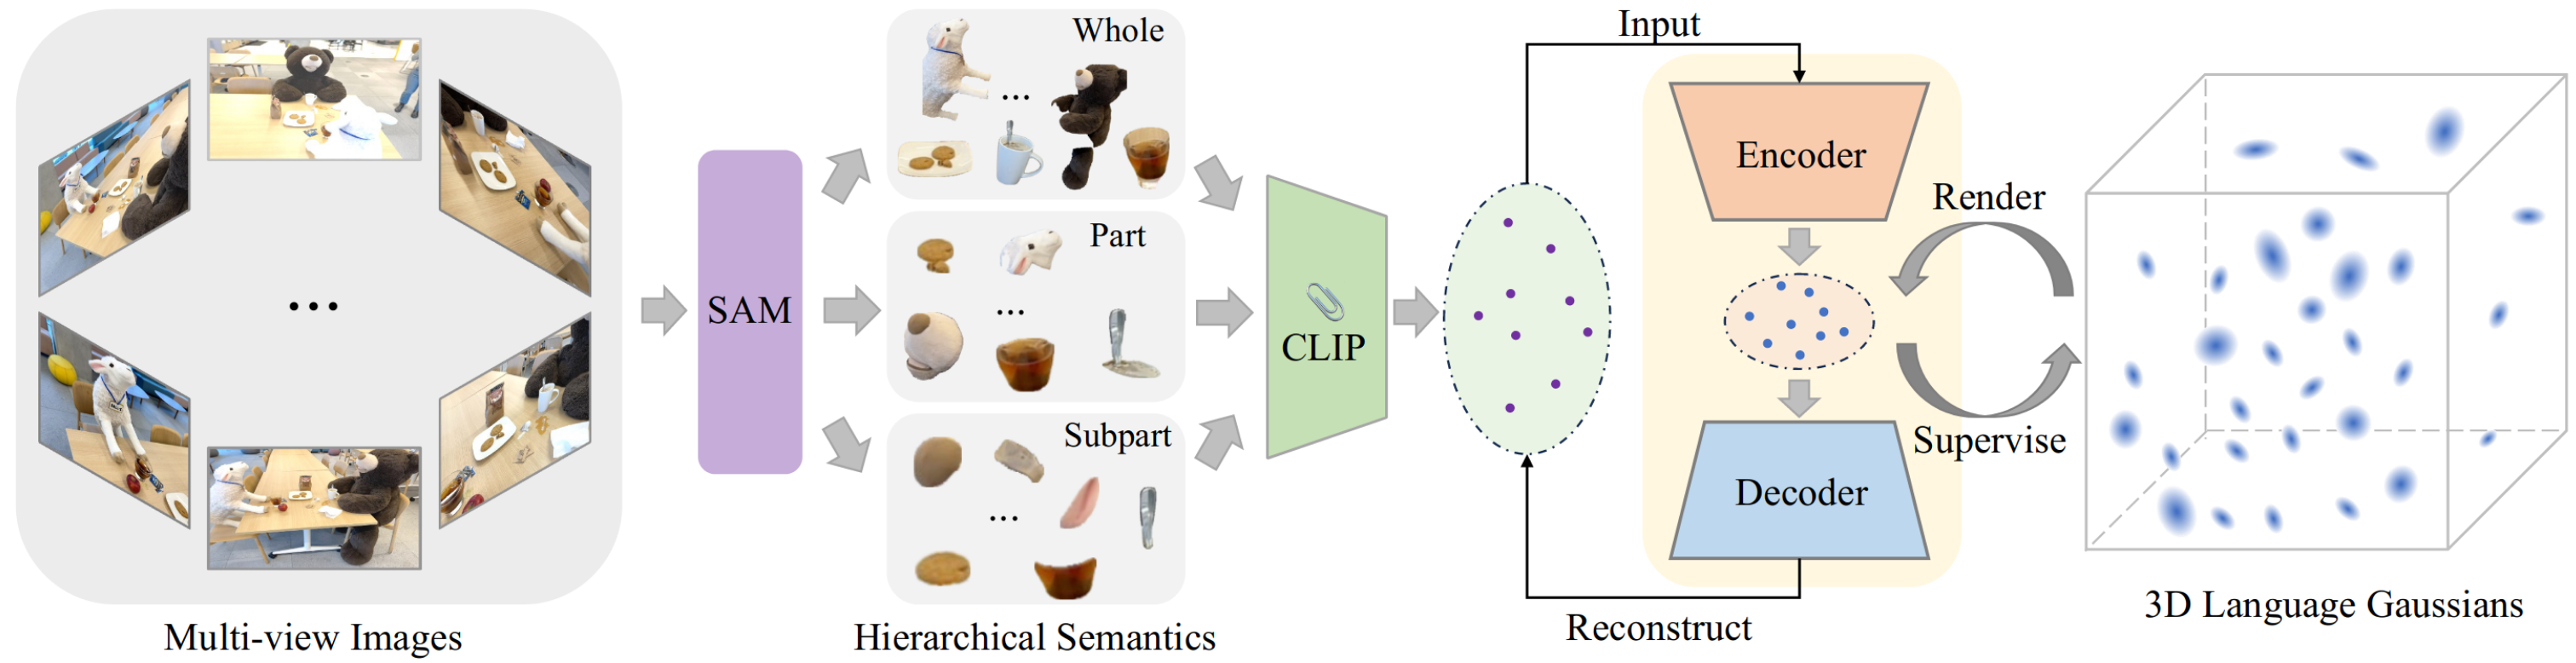
\includegraphics[width=0.8\linewidth]{langsplat-overview.png}}
			\annotatedFigure{0.25,0}{0.55,1}{1}{0.25,0}
			\mode<article>{\annotatedFigure{0.55,0}{0.82,1}{2}{0.55,0}}
		\end{annotatedFigureEnv}
		\caption{Overview of LangSplat}
	\end{figure}
	\mode<presentation>{\vspace*{\fill}}
	\begin{enumerate}[<+(1)->]
		\setlength{\itemsep}{1.5ex}
		\item \alert<.(1)>{Accuracy:} SAM outputs to enhance CLIP features.
		      \mode<presentation>{\vspace*{1.5ex}}
		      \begin{itemize}
			      \mode<presentation>{\setlength{\itemsep}{1.5ex}}
			      \item \alert<.(1)>{CLIP:} image-aligned training leads to ``point-ambiguity''.
			      \item \alert<.(1)>{SAM:} pixel-aligned \& object-centered \& multi-granularity.
		      \end{itemize}
	\end{enumerate}
\end{frame}

\begin{frame}<presentation>
	\mode<presentation>{\Frametitle{Overview}}
	\mode<presentation>{\blfootnote{\href{http://arxiv.org/abs/2312.16084}{(CVPR Highlight, 2024) LangSplat: 3D Language Gaussian Splatting}}}
	\mode<presentation>{
		\begin{figure}[htbp]
			\centering
			\begin{annotatedFigureEnv}
				{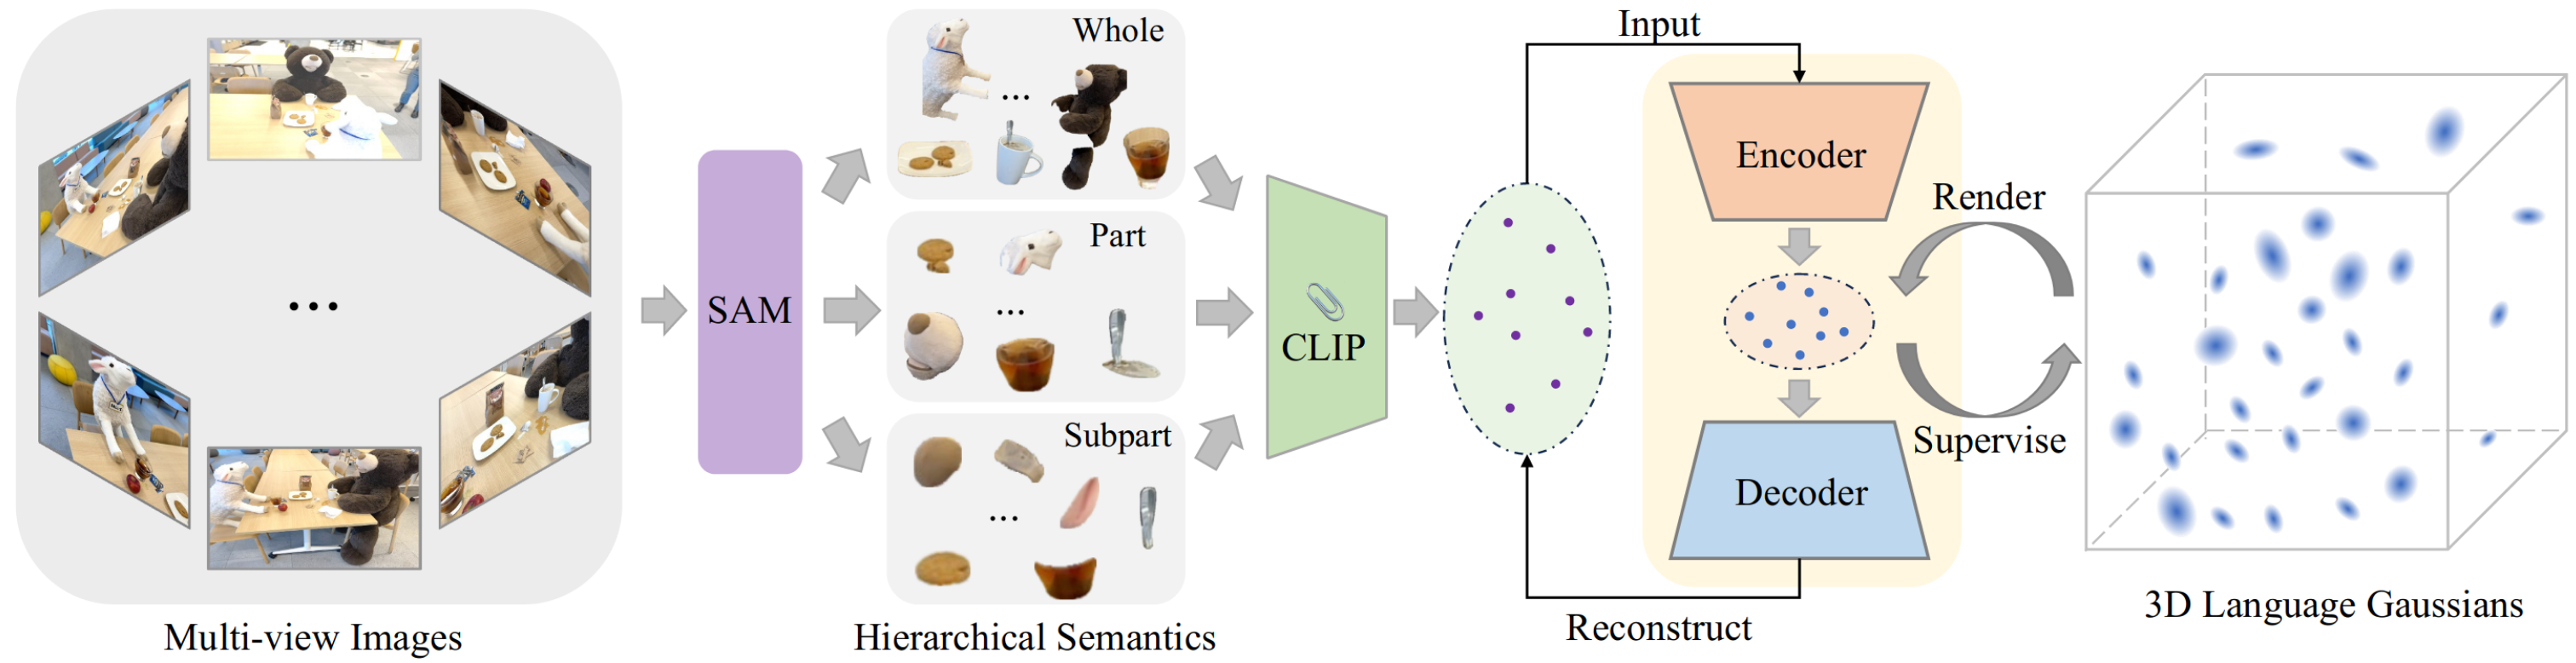
\includegraphics[width=0.8\linewidth]{langsplat-overview.png}}
				\annotatedFigure{0.55,0}{0.82,1}{2}{0.55,0}
			\end{annotatedFigureEnv}
			\addtocounter{figure}{-1}
			\caption{Overview of LangSplat}
		\end{figure}
		\mode<presentation>{\vspace*{\fill}}
	}
	\begin{enumerate}[<+->]
		\mode<presentation>{\setlength{\itemsep}{1.5ex}}
		\setcounter{enumi}{1}
		\item \alert<.>{Efficiency:} an \alert<.>{auto-encoder} to compress latent features.
		      \mode<presentation>{\vspace*{1.5ex}}
		      \begin{itemize}
			      \mode<presentation>{\setlength{\itemsep}{1.5ex}}
			      \item More complexity and better compression,
			            \mode<presentation>{\vspace*{1.5ex}}
			            \par compared with ``speed-up module'' in Feature 3DGS~\autocite{zhouFeature3DGSSupercharging2024apr}.
		      \end{itemize}
	\end{enumerate}
	\blfootnote{In practice, the latent dimension is \(3\) in the auto-encoder.}
\end{frame}

\subsection{CLIP-GS}

\begin{Frame}{Key Insight}
	\begin{figure}[htbp]
		\centering
		\begin{annotatedFigureEnv}
			{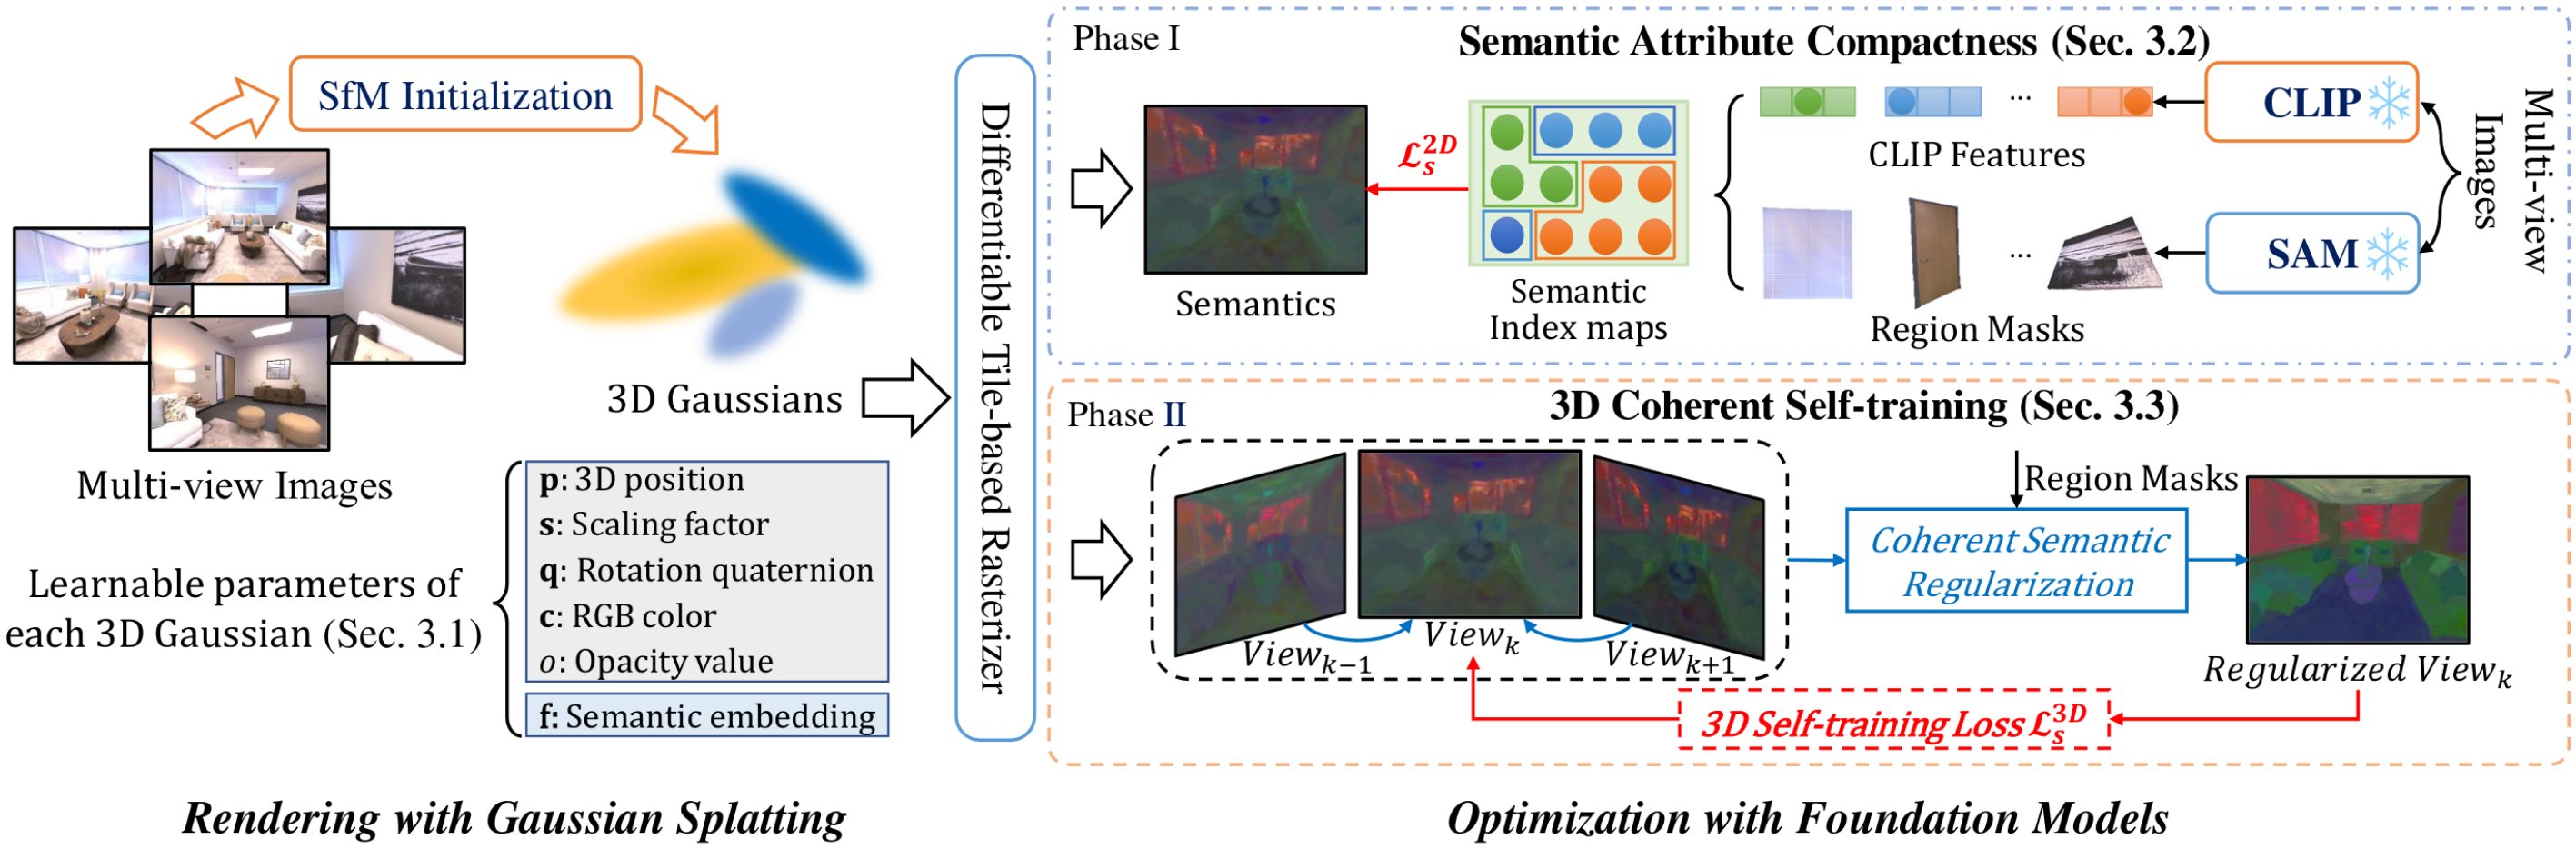
\includegraphics[width=0.7\linewidth]{clip-gs-overview.png}}
			\only<2|handout:1>{\annotatedFigure{0.41,0.57}{1,0.99}{1}{0.41,1.03}}
			\only<3|handout:1>{\annotatedFigure{0.41,0.10}{1,0.55}{2}{0.41,0.58}}
		\end{annotatedFigureEnv}
		\caption{Overview of CLIP-GS}
	\end{figure}
	\begin{enumerate}
		\setlength{\itemsep}{1.5ex}
		\item<2-> \alert<2>{Efficiency:} unify semantic features within an object by leveraging \alert<2>{SAM}.
		\item<3-> \alert<3>{Consistency:} supervise consecutive frames by \alert<3>{video segmentation}.
	\end{enumerate}
	\blfootnote{\href{http://arxiv.org/abs/2404.14249}{(arXiv 04/2024) CLIP-GS: CLIP-informed Gaussian Splatting for Real-time and View-consistent 3D Semantic Understanding}}
\end{Frame}

% \begin{frame}{Methodology: SAC \romannum{1} \hspace{0pt plus 1filll} \small Related Work \(\triangleright\) Semantic 3DGS \(\triangleright\) CLIP-GS}
% 	\colorlet{0_color}{cyan}
% 	\colorlet{0_color_marknode}{0_color!50}
% 	\colorlet{0_color_annotate}{0_color}
% 	\colorlet{1_color}{green}
% 	\colorlet{1_color_marknode}{1_color!50}
% 	\colorlet{1_color_annotate}{1_color}
% 	\vspace*{\fill}
% 	Unify semantic features from CLIP by leveraging SAM,
% 	\begin{figure}[htbp]
% 		\centering
% 		\begin{equation}
% 			\left\{\mathbf{F}^{(0)}, \mathbf{F}^{(1)}, \cdots, \tikzmarknode{index_label}{\colorbox{0_color_marknode}{\(\mathbf{F}^{(m)}\)}}, \cdots, \mathbf{F}^{(M)}\right\}=\operatorname{SAM}\left(\tikzmarknode{semantic-feature-image-clipgs}{\colorbox{1_color_marknode}{\(\mathbf{F}\)}}\right),
% 		\end{equation}
% 		\begin{tikzpicture}[overlay,remember picture,>=stealth,nodes={align=left,inner ysep=1pt},<-]
% 			\path (index_label.north) ++ (0em,0.5em) node[anchor=south east,color=0_color_annotate] (index_label_annotate) { \scriptsize \makecell[l]{\(:=\left\{(i,j,\mathbf{f}^{(m)}) \vert \operatorname{label}(i,j)=m\right\}\)}};
% 			\draw [color=0_color_annotate] (index_label.north) |- (index_label_annotate.south west);
% 			\path (semantic-feature-image-clipgs.north) ++ (0em,0.5em) node[anchor=south west,color=1_color_annotate] (semantic-feature-image-clipgs_annotate) { \scriptsize \makecell[l]{\(\in \mathbb{R}^{H\times W\times D}\)} };
% 			\draw [color=1_color_annotate] (semantic-feature-image-clipgs.north) |- (semantic-feature-image-clipgs_annotate.south east);
% 		\end{tikzpicture}
% 	\end{figure}
% 	where the representative semantic feature is a weighted average,
% 	\begin{equation}
% 		\mathbf{f}^{(m)} := \frac{1}{m} \sum_{(i,\,j)}^{\mathbf{F}^{(m)}} w^{(i,\,j)}\cdot\operatorname{CLIP}\left(\mathbf{c}^{(i,\,j)}\right).
% 	\end{equation}
% 	\vspace*{\fill}
% 	\blfootnote{\href{http://arxiv.org/abs/2404.14249}{[arXiv 04/2024] {CLIP}-{GS}: {CLIP}-informed Gaussian Splatting for Real-time and View-consistent 3D Semantic Understanding}}
% \end{frame}
% 
% \begin{frame}{Methodology: SAC \romannum{2} \hspace{0pt plus 1filll} \small Related Work \(\triangleright\) Semantic 3DGS \(\triangleright\) CLIP-GS}
% 	\colorlet{0_color}{cyan}
% 	\colorlet{0_color_marknode}{0_color!50}
% 	\colorlet{0_color_annotate}{0_color}
% 	\colorlet{1_color}{green}
% 	\colorlet{1_color_marknode}{1_color!50}
% 	\colorlet{1_color_annotate}{1_color}
% 	\vspace*{\fill}
% 	Therefore, we have the semantic index map, i.e. a look-up table,
% 	\begin{figure}[htbp]
% 		\vspace*{-2em}
% 		\centering
% 		\begin{equation}
% 			\mathcal{M}: \tikzmarknode{semantic-index-map}{\colorbox{0_color_marknode}{\(\mathbb{N}_{+}^{H \times W}\)}} \mapsto \tikzmarknode{representative-semantic-feature}{\colorbox{1_color_marknode}{\(\mathbb{R}^{D}\)}}.
% 		\end{equation}
% 		\begin{tikzpicture}[overlay,remember picture,>=stealth,nodes={align=left,inner ysep=1pt},<-]
% 			\path (semantic-index-map.south) ++ (0em,-1em) node[anchor=north east,color=0_color_marknode] (semantic-index-map_annotate) { \scriptsize \makecell[l]{semantic index map} };
% 			\draw [color=0_color_marknode] (semantic-index-map.south) |- (semantic-index-map_annotate.south west);
% 			\path (representative-semantic-feature.south) ++ (0em,-1em) node[anchor=north west,color=1_color_marknode] (representative-semantic-feature_annotate) { \scriptsize \makecell[l]{representative semantic feature} };
% 			\draw [color=1_color_marknode] (representative-semantic-feature.south) |- (representative-semantic-feature_annotate.south east);
% 		\end{tikzpicture}
% 	\end{figure}
% 	\vspace*{\fill}
% 	\par We learn the semantic index map, instead of semantic features, by leveraging
% 	\vspace*{1.5ex}
% 	\begin{enumerate}
% 		\setlength{\itemsep}{1.5ex}
% 		\item super low-dimensional Gaussian-wise embeddings, e.g. \(\dim= 3\);
% 		\item a classification head.
% 	\end{enumerate}
% 	\vspace*{\fill}
% \end{frame}
% 
% % \begin{frame}{Methodology: 3DCS \hspace{0pt plus 1filll} \small Related Work \(\triangleright\) Semantic 3DGS \(\triangleright\) CLIP-GS}
% % 	\vspace*{\fill}
% % 	TODO
% % 	% \par Use a pre-trained video tracker to associate SAM masks across consecutive frames.
% % 	\vspace*{\fill}
% % \end{frame}
% % 
% % \begin{frame}{Methodology: Training \hspace{0pt plus 1filll} \small Related Work \(\triangleright\) Semantic 3DGS \(\triangleright\) CLIP-GS}
% % 	\vspace*{\fill}
% % 	TODO
% % 	\vspace*{\fill}
% % \end{frame}
% 
% \begin{frame}{Limitations \hspace{0pt plus 1filll} \small Related Work \(\triangleright\) Semantic 3DGS \(\triangleright\) CLIP-GS}
% 	\vspace*{\fill}
% 	\begin{enumerate}
% 		\setlength{\itemsep}{3em}
% 		\item SAM is not perfect.
% 		      \vspace*{1.5ex}
% 		      \begin{itemize}
% 			      \setlength{\itemsep}{1.5ex}
% 			      \item What happens if masks are inaccurate?
% 			      \item How can we choose an adequate granularity adaptively?
% 		      \end{itemize}
% 		\item 3D consistency is maintained locally, not globally.
% 		      \vspace*{1.5ex}
% 		      \begin{itemize}
% 			      \setlength{\itemsep}{1.5ex}
% 			      \item A 2D video segmentation model can only supervise consecutive frames.
% 		      \end{itemize}
% 	\end{enumerate}
% 	\vspace*{\fill}
% \end{frame}
% 
% \subsubsection*{RT-GS2}
% \begin{frame}{Overview\hspace{0pt plus 1filll} \small Related Work \(\triangleright\) Semantic 3DGS \(\triangleright\) RT-GS2}
% 	\vspace*{\fill}
% 	\begin{block}{Key Insight}
% 		\par Learn view-indenpendent semantic features by self-supervision to enhance 3D consistency.
% 	\end{block}
% 	\vspace*{\fill}
% 	\begin{figure}[htbp]
% 		\begin{minipage}[c]{0.35\linewidth}
% 			\centering
% 			\includegraphics[width=\linewidth]{rt-gs2-overview.png}
% 		\end{minipage}
% 		\vspace*{\fill}
% 		\begin{minipage}[c]{0.60\linewidth}
% 			\begin{enumerate}
% 				\setlength{\itemsep}{3ex}
% 				\item \textbf{V}iew-\textbf{I}ndenpendent \textbf{F}eature:\\[1.5ex]
% 				      leverage an auto-encoder for contrastive learning across multi-views.
% 				\item \textbf{V}iew-\textbf{I}ndenpendent \& \textbf{V}iew-\textbf{D}enpendent \textbf{F}eature \textbf{F}usion
% 			\end{enumerate}
% 		\end{minipage}
% 	\end{figure}
% 	\vspace*{\fill}
% \end{frame}

% \subsubsection*{CoSSegGaussians}
% \begin{frame}{Overview \hspace{0pt plus 1filll} \small Related Work \(\triangleright\) Semantic 3DGS \(\triangleright\) CoSSegGaussians}
% 	\vspace*{\fill}
% 	\begin{block}{Key Insight}
% 		\par
% 	\end{block}
% 	\vspace*{\fill}
% 	\begin{figure}[htbp]
% 		\begin{minipage}[c]{0.35\linewidth}
% 			\centering
% 			\includegraphics[width=\linewidth]{cosseggaussians-overview.png}
% 		\end{minipage}
% 		\hspace{\fill}
% 		\begin{minipage}[c]{0.60\linewidth}
% 			\centering
% 			\begin{enumerate}
% 				\setlength{\itemsep}{1.5ex}
% 				\item Hello
% 			\end{enumerate}
% 		\end{minipage}
% 	\end{figure}
% \end{frame}
% 
% 
% \subsubsection*{Fast-LGS}
% \begin{frame}{Overview \hspace{0pt plus 1filll} \small Related Work \(\triangleright\) Semantic 3DGS \(\triangleright\) Fast-LGS}
% 	\vspace*{\fill}
% 	TODO
% 	\vspace*{\fill}
% \end{frame}
% \begin{frame}{Methodology: \hspace{0pt plus 1filll} \small Related Work \(\triangleright\) Semantic 3DGS \(\triangleright\) Fast-LGS}
% 	\vspace*{\fill}
% 	\begin{block}{Motivation}
% 		A vanilla integration of Gaussian-wise CLIP features,
% 		\begin{enumerate}
% 			\setlength{\itemsep}{1.5ex}
% 			\item computation \& memory inefficiency
% 			\item inconsistency and inaccuracy
% 		\end{enumerate}
% 		MLP-based compression
% 	\end{block}
% 	\vspace*{\fill}
% \end{frame}


%!Tex Root=**/main.tex

\mode<article>{\chapter{3DGS SLAM}}
\mode<presentation>{\section{3DGS SLAM}}

\mode<article>{\section{Overview}}
\mode<presentation>{\subsection{Overview}}

\begin{frame}\Frametitle{Research Background}
	\colorlet{accepted}{ForestGreen}
	\mode<article>{\par Figure~\ref{fig:3dgs-slam-timeline} shows the timeline of 3DGS SLAM research.}
	\begin{figure}[htbp]
		\centering
		\begin{tikzpicture}
			\usetikzlibrary{calc}
			\usetikzlibrary{positioning}

			\pgfmathsetmacro{\dy}{0.3cm/1pt};
			\pgfmathsetmacro{\nodeNum}{3};
			\pgfmathsetmacro{\sepNum}{\nodeNum-1};
			\pgfmathsetmacro{\length}{0.8*\linewidth};
			\pgfmathsetmacro{\edgeLength}{1cm/1pt};
			\pgfmathsetmacro{\dx}{(\length-\edgeLength-\edgeLength)/\sepNum};
			\pgfmathsetmacro{\xShift}{0};

			\mode<article>{\tikzset{
					node distance=1.5ex,
					note/.style={ anchor=north, align=center, text width=\dx, yshift=-\dy/3, font={\small\sffamily} },
					time/.style={ anchor=south, font={\small\sffamily} },
				}}

			\mode<presentation>{\tikzset{
					node distance=1.5ex,
					note/.style={ anchor=north, align=center, text width=\dx, yshift=-\dy/3, font={\scriptsize\sffamily} },
					time/.style={ anchor=south, font={\scriptsize\sffamily} },
				}}

			\coordinate (start) at (0 pt,0 pt);
			\coordinate (end) at (\length pt,0 pt);
			\draw [line width=1.5pt,-stealth] (start) -- (end);

			\foreach \counter in {0,...,\sepNum} {
					\coordinate (s\counter) at (\edgeLength+\counter*\dx pt,0);
					\coordinate (t\counter) at ($(s\counter)+(0,\dy pt)$);
					\draw [line width=1.5pt] (s\counter) -- (t\counter);
				}

			\node [time] at (t0.north) { 11/2023 - 12/2024 };
			\node [note, below of= s0] (s0_1) { \textcolor{accepted}{SplaTAM}~\autocite{keetha_splatam_2024} };
			\node [note, below of= s0_1] (s0_2) { \textcolor{accepted}{GS-SLAM}~\autocite{yan_gs-slam_2023} };
			\node [note, below of= s0_2] (s0_3) { Gaussian-SLAM~\autocite{yugay_gaussian-slam_2024} };
			\node [note, below of= s0_3] (s0_4) {\textcolor{accepted}{MonoGS}~\autocite{matsuki_gaussian_2024}};
			\node [time] at (t1.north) { 01/2024 - 04/2024 };
			\node [note, below of=s1] (s1_1) {\textcolor{accepted}{RTG-SLAM}~\autocite{peng_rtg-slam_2024}};
			\node [time] at (t2.north) { 05/2024 - 06/2024 };
		\end{tikzpicture}
		\vspace*{0.5ex}
		\caption[Timeline of 3DGS SLAM research]{Timeline of 3DGS SLAM research (\textcolor{accepted}{accepted})}
		\label{fig:3dgs-slam-timeline}
	\end{figure}
\end{frame}

%!Tex Root=**/main.tex

\section{MonoGS}

\subsection{Methodology}

\begin{Frame}{Overview \romannum{1}}
	\begin{figure}[htbp]
		\centering
		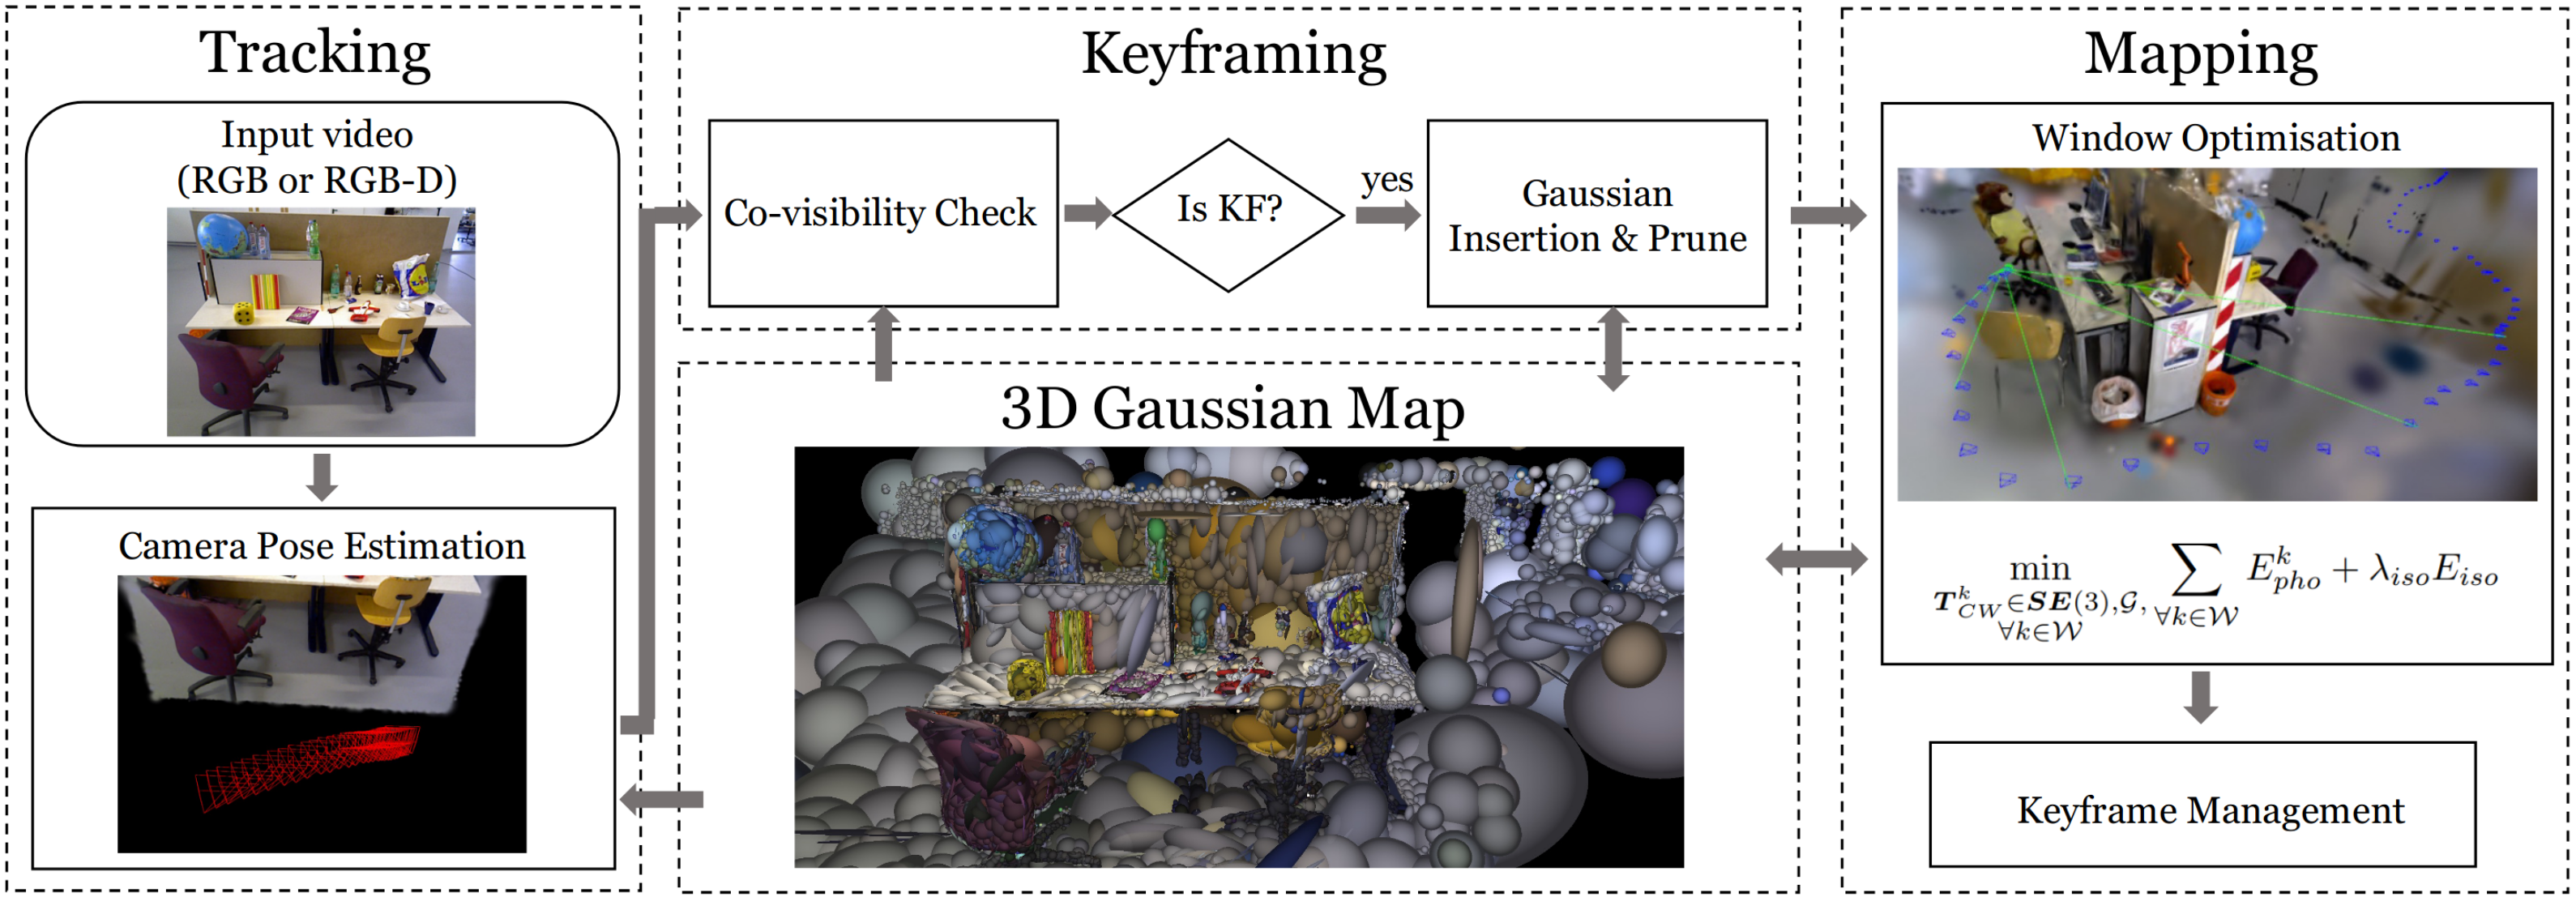
\includegraphics[width=\linewidth]{monogs/overview.png}
	\end{figure}
	\blfootnote{\href{http://arxiv.org/abs/2312.06741}{(CVPR Highlight, 2024) MonoGS: Gaussian Splatting SLAM}}
\end{Frame}

\tikzset{
	key/.style={
			draw=OrangeRed,
		},
	convention/.style={
			draw=Cerulean,
		},
	trick/.style={
			draw=ForestGreen,
		},
}
\begin{Frame}{Overview \romannum{2}}
	\centering
	\resizebox{0.85\textwidth}{!}{
		\begin{forest}
			for tree={my tree}
			[
			MonoGS
				[
					Visual Odometry,for children={visible on=<1->}
						[
							Tracking,for children={visible on=<2->}
								[
									``Inverse Rendering'',for children={visible on=<3->}
										[
											Analytical Jacobians Derivation,key
										]
										[
											Photometric RGB \& Depth Loss,convention
										]
										[
											Optimizable Exposure,trick
										]
										[
											Penalization on non-edge/low-opacity pixels,trick
										]
								]
						]
						[
							Mapping,for children={visible on=<2->}
								[
									Bundle Adjustment,for children={visible on=<3->}
										[
											Photometric RGB \& Depth Loss,convention
										]
										[
											Isotropic Regularization,key
										]
										[
											Random Recall,trick
										]
								]
						]
				]
				[
					Online Pipeline,for children={visible on=<1->}
						[
							Keyframe Management,for children={visible on=<2->}
								[
									Registration,for children={visible on=<3->}
										[
											Gaussian Covisibility,key
										]
										[
											Relative Translation,convention
										]
								]
								[
									Removal,for children={visible on=<3->}
										[
											Gaussian Overlap Coefficient,key
										]
								]
						]
						[
							Gaussian Management,for children={visible on=<2->}
								[
									Insertion,for children={visible on=<3->}
										[
											Keyframing,convention
										]
								]
								[
									Pruning,for children={visible on=<3->}
										[
											Gaussian Covisibility,key
										]
								]
						]
				]
			]
		\end{forest}
	}
	\resizebox{0.08\textwidth}{!}{
		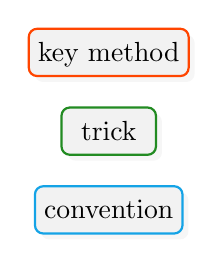
\begin{tikzpicture}[visible on=<3->]
			\node [my node for tree, draw=ForestGreen] (trick node) {trick};
			\node [my node for tree, draw=OrangeRed, above of = trick node] {key method};
			\node [my node for tree, draw=Cerulean, below of = trick node] (convention) {convention};
		\end{tikzpicture}
	}
	\blfootnote{\href{http://arxiv.org/abs/2312.06741}{(CVPR Highlight, 2024) MonoGS: Gaussian Splatting SLAM}}
\end{Frame}

\begin{Frame}{Tracking: Overview}
	\begin{figure}[htbp]
		\centering
		\resizebox{0.7\textwidth}{!}{
			\begin{forest} for tree={my tree}
				[
				Tracking
				[
				``Inverse Rendering''
				[
				Analytical Jacobians Derivation,key
				]
				[
				Photometric RGB \& Depth Loss,convention
				]
				[
				Optimizable Exposure,trick
				]
				[
				Penalization on non-edge/low-opacity pixels,trick
				]
				]
				]
			\end{forest}
		}
	\end{figure}
	\vspace*{\fill}
	\par Track camera poses,
	\vspace*{1.5ex}
	\begin{itemize}[<+->]
		\setlength{\itemsep}{1.5ex}
		\item \textcolor{OrangeRed}{through the extended differentiable rendering pipeline},
		\item \textcolor{Cerulean}{by a direct optimization against fixed 3D Gaussians,}
		\item \textcolor{ForestGreen}{with some tricks to be more adaptive to brightness and more robust to noise.}
	\end{itemize}
	\blfootnote{
		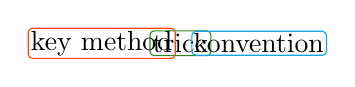
\begin{tikzpicture}
			\node [inner sep=1pt, rounded corners=1.5, draw=ForestGreen] (trick node) {trick};
			\node [inner sep=1pt, rounded corners=1.5, draw=OrangeRed, left of = trick node] {key method};
			\node [inner sep=1pt, rounded corners=1.5, draw=Cerulean, right of = trick node] (convention) {convention};
		\end{tikzpicture}
	}
	\blfootnote{\href{http://arxiv.org/abs/2312.06741}{(CVPR Highlight, 2024) MonoGS: Gaussian Splatting SLAM}}
\end{Frame}

\begin{Frame}{Tracking: A Review of 3DGS}
	\vspace*{-5em}
	\par The projection from ``ellipsoids'' to ``ellipses'' in 3DGS,
	\begin{equation}
		\mathcal{N}\left(\mu_w, \Sigma_w\right) \overset{\pi}{\mapsto} \mathcal{N}\left(\mu_i, \Sigma_i\right),
	\end{equation}
	is achieved by,
	\begin{overprint}[\textheight]
		\begin{figure}[htbp]
			\centering
			\begin{minipage}[c]{0.35\linewidth}
				\resetcolorseries[4]{marknode-color-series}
				\resetcolorseries[4]{annotation-color-series}
				\begin{align}
					\alt<5->{\tikzmarknode{n3}{\colorbox{marknode-color-series!![3]}{\(\mu_{i}\)}}}{\mu_{i}}
					=
					\alt<4->{\tikzmarknode{n2}{\colorbox{marknode-color-series!![2]}{\(\pi\)}}}{\pi}
					\left(
					\alt<3->{\tikzmarknode{n1}{\colorbox{marknode-color-series!![1]}{\(\mathbf{T}_{cw}\)}}}{\mathbf{T}_{cw}}
					\cdot
					\alt<2->{\tikzmarknode{n0}{\colorbox{marknode-color-series!![0]}{\(\mu_{w}\)}}}{\mu_{w}}
					\right)
				\end{align}
				\begin{annotatedEquationEnv}
					\only<2->{\annotatedEquation{colorseries}{n0}{south}{0em}{-1em}{north west}{annotation-color-series}{\(\in \mathbb{P}^3\), 3D(world) mean}{east}}
					\only<3->{\annotatedEquation{colorseries}{n1}{south}{0em}{-3em}{north west}{annotation-color-series}{\(\in \mathrm{SE}(3)\), camera pose}{east}}
					\only<4->{\annotatedEquation{colorseries}{n2}{south}{0em}{-5em}{north west}{annotation-color-series}{projection}{east}}
					\only<5->{\annotatedEquation{colorseries}{n3}{south}{0}{-7em}{north west}{annotation-color-series}{\(\in \mathbb{P}^2\), 2D(image) mean}{east}}
				\end{annotatedEquationEnv}
			\end{minipage}
			\begin{minipage}[c]{0.60\linewidth}
				\resetcolorseries[4]{marknode-color-series}
				\resetcolorseries[4]{annotation-color-series}
				\begin{align}
					\alt<9->{\tikzmarknode{n3}{\colorbox{marknode-color-series!![3]}{\(\Sigma_{i}\)}}}{\Sigma_{i}}
					=
					\alt<8->{\tikzmarknode{n2}{\colorbox{marknode-color-series!![2]}{\(\mathbf{J}_{\pi}\)}}}{\mathbf{J}_{\pi}}
					\alt<7->{\tikzmarknode{n1}{\colorbox{marknode-color-series!![1]}{\(\mathbf{R}_{cw}\)}}}{\mathbf{R}_{cw}}
					\alt<6->{\tikzmarknode{n0}{\colorbox{marknode-color-series!![0]}{\(\Sigma_{w}\)}}}{\Sigma_{w}}  \mathbf{R}_{cw}^{\mathrm{T}} \mathbf{J}_{\pi}^{\mathrm{T}}
				\end{align}
				\begin{annotatedEquationEnv}
					\only<6->{\annotatedEquation{colorseries}{n0}{south}{0em}{-1em}{north west}{annotation-color-series}{\(\in \mathbb{R}^{3\times 3}\), 3D(world) covariance}{east}}
					\only<7->{\annotatedEquation{colorseries}{n1}{south}{0em}{-3em}{north west}{annotation-color-series}{\(\in \mathrm{SO(3)}\), rotation component of \(\mathbf{T}_{cw}\)}{east}}
					\only<8->{\annotatedEquation{colorseries}{n2}{south}{0em}{-5em}{north west}{annotation-color-series}{\(\in \mathbb{R}^{2\times 3}\), Jacobian of the linear approximation of \(\pi\)}{east}}
					\only<9->{\annotatedEquation{colorseries}{n3}{south}{0em}{-7em}{north west}{annotation-color-series}{\(\in \mathbb{R}^{2\times 2}\), 2D(image) covariance}{east}}
				\end{annotatedEquationEnv}
			\end{minipage}
		\end{figure}
	\end{overprint}
	\blfootnote{\href{http://arxiv.org/abs/2312.06741}{(CVPR Highlight, 2024) MonoGS: Gaussian Splatting SLAM}}
\end{Frame}

\begin{Frame}{Tracking: Derivation of Jacobians \romannum{1}}
	\par The chain rule,
	\begin{alignat}{1}
		\frac{\partial \mu_i}{\partial \mathbf{T}_{cw}}    & = \frac{\partial \mu_i}{\partial \mu_c} \frac{\partial \mu_c}{\partial \mathbf{T}_{cw}}                                                                                                                                                                               \\
		\frac{\partial \Sigma_i}{\partial \mathbf{T}_{cw}} & = \frac{\partial \Sigma_i}{\partial \mathbf{J}_{\pi}} \frac{\partial \mathbf{J}_{\pi}}{\partial \mu_c} \frac{\partial \mu_c}{\partial \mathbf{T}_{cw}} + \frac{\partial \Sigma_i}{\partial \mathbf{R}_{cw}} \frac{\partial \mathbf{R}_{cw}}{\partial \mathbf{T}_{cw}}
	\end{alignat}
	\pause
	\par The Lie Algebra,
	\begin{alignat}{1}
		\frac{\partial \mu_c}{\partial \mathbf{T}_{cw}}           & = \begin{bmatrix}
			                                                              \mathbf{I} & -\mu_{c}^{\times}
		                                                              \end{bmatrix}               \\
		\frac{\partial \mathbf{R}_{cw}}{\partial \mathbf{T}_{cw}} & = \begin{bmatrix}
			                                                              \mathbf{0} & - \mathbf{R}_{cw}^{\times}(:,1) \\
			                                                              \mathbf{0} & - \mathbf{R}_{cw}^{\times}(:,2) \\
			                                                              \mathbf{0} & - \mathbf{R}_{cw}^{\times}(:,3) \\
		                                                              \end{bmatrix}
	\end{alignat}
	\blfootnote{\href{http://arxiv.org/abs/2312.06741}{(CVPR Highlight, 2024) MonoGS: Gaussian Splatting SLAM}}
\end{Frame}

\begin{Frame}{Online Pipeline: Overview}
	\begin{figure}[htbp]
		\centering
		\resizebox{0.8\textwidth}{!}{
			\begin{forest}
				for tree={my tree}
				[
				Online Pipeline
					[
						Keyframe Management
							[
								Registration
									[
										Gaussian Covisibility,key
									]
									[
										Relative Translation,convention
									]
							]
							[
								Removal
									[
										Gaussian Overlap Coefficient,key
									]
							]
					]
					[
						Gaussian Management
							[
								Insertion
									[
										Keyframing,convention
									]
							]
							[
								Pruning
									[
										Gaussian Covisibility,key
									]
							]
					]
				]
			\end{forest}
		}
	\end{figure}
	\par \alert<+|handout:0>{Keyframe Management}:
	\vspace*{1.5ex}
	\begin{itemize}[<+->]
		\setlength{\itemsep}{1.5ex}
		\item \alert<.|handout:0>{Classic} strategies, e.g. covisibility \& overlap, from DSO~\autocite{engel2016dso}.
		\item \alert<.|handout:0>{Off-the-shelf} occlusion-aware Gaussian visibility is leveraged to construct metrics.
	\end{itemize}
	\blfootnote{
		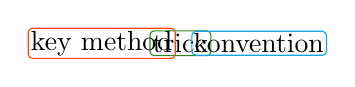
\begin{tikzpicture}
			\node [inner sep=1pt, rounded corners=1.5, draw=ForestGreen] (trick node) {trick};
			\node [inner sep=1pt, rounded corners=1.5, draw=OrangeRed, left of = trick node] {key method};
			\node [inner sep=1pt, rounded corners=1.5, draw=Cerulean, right of = trick node] (convention) {convention};
		\end{tikzpicture}
	}
	\blfootnote{\href{http://arxiv.org/abs/1607.02565}{(arXiv, 2016) DSO: Direct Sparse Odometry}}
	\blfootnote{\href{http://arxiv.org/abs/2312.06741}{(CVPR Highlight, 2024) MonoGS: Gaussian Splatting SLAM}}
\end{Frame}

\begin{Frame}{Online Pipeline: Overview}
	\begin{figure}[htbp]
		\centering
		\resizebox{0.8\textwidth}{!}{
			\begin{forest}
				for tree={my tree}
				[
				Online Pipeline
					[
						Keyframe Management
							[
								Registration
									[
										Gaussian Covisibility,key
									]
									[
										Relative Translation,convention
									]
							]
							[
								Removal
									[
										Gaussian Overlap Coefficient,key
									]
							]
					]
					[
						Gaussian Management
							[
								Insertion
									[
										Keyframing,convention
									]
							]
							[
								Pruning
									[
										Gaussian Covisibility,key
									]
							]
					]
				]
			\end{forest}
		}
	\end{figure}
	\par \alert<+|handout:0>{Gaussian Management:}
	\vspace*{1.5ex}
	\begin{itemize}[<+->]
		\setlength{\itemsep}{1.5ex}
		\item \alert<.>{Insertion:} triggered by \alert<.>{keyframing}, followed by \alert<.>{Gaussian initialization}.
		\item \alert<.>{Pruning:} to remove unstable/incorrect Gaussians by covisibility in a monocular setting.
	\end{itemize}
	\blfootnote{
		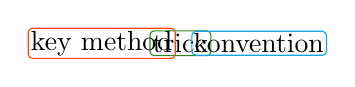
\begin{tikzpicture}
			\node [inner sep=1pt, rounded corners=1.5, draw=ForestGreen] (trick node) {trick};
			\node [inner sep=1pt, rounded corners=1.5, draw=OrangeRed, left of = trick node] {key method};
			\node [inner sep=1pt, rounded corners=1.5, draw=Cerulean, right of = trick node] (convention) {convention};
		\end{tikzpicture}
	}
	\blfootnote{\href{http://arxiv.org/abs/1607.02565}{(arXiv, 2016) DSO: Direct Sparse Odometry}}
	\blfootnote{\href{http://arxiv.org/abs/2312.06741}{(CVPR Highlight, 2024) MonoGS: Gaussian Splatting SLAM}}
\end{Frame}

\begin{Frame}{Keyframe Management: Prerequistes}
	\begin{enumerate}
		\setlength{\itemsep}{3ex}
		\item<+-> \alert<.>{What} is keyframing or keyframe management?
			\vspace*{1.5ex}
			\begin{itemize}
				\setlength{\itemsep}{1.5ex}
				\item<+-> A strategy of \alert<.>{selecting} and \alert<.>{utilizing} a \alert<.>{crucial subset} of frames.
			\end{itemize}
		\item<+-> \alert<.>{Why} do we need keyframing?
			\vspace*{1.5ex}
			\begin{itemize}
				\setlength{\itemsep}{1.5ex}
				\item<+-> \alert<.>{Infeasible} to optimize jointly on all frames online.
					\vspace*{1.5ex}
					\visible<+->{\par (a \alert<.>{trade-off} between efficiency and accuracy/robustness/...)}
			\end{itemize}
		\item<+-> \alert<.>{How} should we select keyframes?
			\vspace*{1.5ex}
			\begin{itemize}
				\setlength{\itemsep}{1.5ex}
				\item<+-> \alert<.>{non-redundant} and observing the \alert<.>{same area}.
				\item<+-> spanning a \alert<.>{wide baseline} for better multi-view constraints.
			\end{itemize}
	\end{enumerate}
	\blfootnote{\href{http://arxiv.org/abs/2312.06741}{(CVPR Highlight, 2024) MonoGS: Gaussian Splatting SLAM}}
\end{Frame}

\begin{Frame}{Keyframe Management: Registration}
	\blfootnote{\href{http://arxiv.org/abs/2312.06741}{(CVPR Highlight, 2024) MonoGS: Gaussian Splatting SLAM}}
	\begin{overprint}[\textheight]
		\par If \alert<+>{any} of the following conditions \alert<.>{is true}...
		\vspace*{\fill}
		\resetcolorseries[6]{marknode-color-series}
		\resetcolorseries[6]{annotation-color-series}
		\begin{block}<+->{\alert<.|handout:0>{Small Gaussian Covisibility}\hfill Condition \romannum{1}, Keyframe Registration}
			Gaussian covisibility between the current frame and the previous keyframe drops below a threshold.
			\begin{figure}[htbp]
				\centering
				\begin{onlyenv}<.>
					\vspace*{-2em}
					\begin{equation*}
						\frac{\vert\operatorname{v}\left(\mathcal{G}, \mathcal{F}_{i}\right) \cap \tikzmarknode{n0}{\colorbox{marknode-color-series!![0]}{\(\operatorname{v}\left(\mathcal{G}, \mathcal{F}_{j}\right)\)}} \vert}{\vert\operatorname{v}\left(\mathcal{G}, \tikzmarknode{n1}{\colorbox{marknode-color-series!![1]}{\(\mathcal{F}_{i}\)}}\right) \cup \operatorname{v}\left(\mathcal{G}, \tikzmarknode{n2}{\colorbox{marknode-color-series!![2]}{\(\mathcal{F}_{j}\)}}\right) \vert} < \tau_1
					\end{equation*}
					\begin{annotatedEquationEnv}
						\annotatedEquation{colorseries}{n0}{north}{0em}{1em}{south west}{annotation-color-series}{\(\subset \mathcal{G}\), \textbf{visible} Gaussians from frame \(j\)}{east}
						\annotatedEquation{colorseries}{n1}{south}{0em}{-0.5em}{north east}{annotation-color-series}{the previous keyframe}{west}
						\annotatedEquation{colorseries}{n2}{south}{0em}{-0.5em}{north west}{annotation-color-series}{the current frame}{east}
					\end{annotatedEquationEnv}
				\end{onlyenv}
				\begin{onlyenv}<+-|handout:0>
					\vspace*{-2em}
					\begin{equation}
						\frac{\vert\operatorname{v}\left(\mathcal{G}, \mathcal{F}_{i}\right) \cap \operatorname{v}\left(\mathcal{G}, \mathcal{F}_{j}\right) \vert}{\vert\operatorname{v}\left(\mathcal{G}, \mathcal{F}_{i}\right) \cup \operatorname{v}\left(\mathcal{G}, \mathcal{F}_{j}\right) \vert} < \tau_1
					\end{equation}
					\vspace*{-2em}
				\end{onlyenv}
			\end{figure}
		\end{block}
		\vspace*{\fill}
		\begin{block}<.->{\alert<.|handout:0>{Large Relative Translation}\hfill Condition \romannum{2}, Keyframe Registration}
			Translation from the previous keyframe w.r.t. to the median depth reaches a threshold.
			\begin{figure}[htbp]
				\centering
				\vspace*{-2em}
				\begin{onlyenv}<.>
					\begin{equation*}
						\frac{\Vert \mathbf{t}_{\mathcal{F}_i \mathcal{F}_j} \Vert_2}{\bar{D}_{\mathcal{F}_i \mathcal{F}_j}} > \tau_2, \quad \bar{D}_{\mathcal{F}_i \mathcal{F}_j} = \frac{1}{2 \tikzmarknode{n4}{\colorbox{marknode-color-series!![4]}{\(H\)}} \tikzmarknode{n5}{\colorbox{marknode-color-series!![5]}{\(W\)}}} \sum^{\{\mathcal{F}_i,\mathcal{F}_j\}} \sum_{h=0}^{H} \sum_{w=0}^{W} \tikzmarknode{n3}{\colorbox{marknode-color-series!![3]}{\(d(h,w)\)}}
					\end{equation*}
					\begin{annotatedEquationEnv}
						\annotatedEquation{colorseries}{n3}{south}{0}{-0.5em}{north west}{annotation-color-series}{depth of pixel \((h,w)\)}{east}
						\annotatedEquation{colorseries}{n4}{south}{0}{-0.5em}{north east}{annotation-color-series}{image height}{west}
						\annotatedEquation{colorseries}{n5}{south}{0}{-0.5em}{north west}{annotation-color-series}{image width}{east}
					\end{annotatedEquationEnv}
				\end{onlyenv}
				\begin{onlyenv}<+-|handout:0>
					\begin{equation}
						\frac{\Vert \mathbf{t}_{\mathcal{F}_i \mathcal{F}_j} \Vert_2}{\bar{D}_{\mathcal{F}_i \mathcal{F}_j}} > \tau_2, \quad \bar{D}_{\mathcal{F}_i \mathcal{F}_j} = \frac{1}{2 H W} \sum^{\{\mathcal{F}_i,\mathcal{F}_j\}} \sum_{h=0}^{H} \sum_{w=0}^{W} d(h,w)
					\end{equation}
					\vspace*{-2em}
				\end{onlyenv}
			\end{figure}
		\end{block}
	\end{overprint}
\end{Frame}

\begin{Frame}{Keyframe Management: Removal}
	\blfootnote{\href{http://arxiv.org/abs/2312.06741}{(CVPR Highlight, 2024) MonoGS: Gaussian Splatting SLAM}}
	\begin{overprint}[\textheight]
		\par If \alert<+>{any} of the following conditions \alert<.>{is true}...
		\vspace*{\fill}
		\begin{block}{\alert<.|handout:0>{Beyond Window Capacity}\hfill Condition \romannum{1}, Keyframe Removal}<+->
			Remove the earliest keyframe out of the sliding window if the capacity is exceeded.
			\begin{equation}
				\vert \mathcal{W} \vert < \tau_3
			\end{equation}
		\end{block}
		\vspace*{\fill}
		\begin{block}{\alert<.|handout:0>{Low Gaussian Overlap Coefficient}\hfill Condition \romannum{2}, Keyframe Removal}<+->
			Remove the previous keyframe if the ``Gaussian overlap coefficient'' between the previous frame and the new keyframe drops below a threshold.
			\begin{equation}
				\frac{\vert \operatorname{v}\left(\mathcal{G}, \mathcal{F}_{i}\right) \cap \operatorname{v}\left(\mathcal{G}, \mathcal{F}_{j}\right) \vert}{\min \left(\vert\operatorname{v}\left(\mathcal{G}, \mathcal{F}_{i}\right) \vert, \vert\operatorname{v}\left(\mathcal{G}, \mathcal{F}_{j}\right) \vert\right)} < \tau_4
			\end{equation}
		\end{block}
	\end{overprint}
\end{Frame}

\begin{Frame}{Gaussian Management: Insertion}
	\begin{itemize}
		\setlength{\itemsep}{1.5ex}
		\item<+-> \alert<.>{Why} do we need ``Gaussian insertion''?
			\vspace*{1.5ex}
			\begin{itemize}
				\setlength{\itemsep}{1.5ex}
				\item<+-> \alert<.>{SLAM} is for robotic exploration.
			\end{itemize}
	\end{itemize}
	\vspace*{\fill}
	\begin{itemize}
		\setlength{\itemsep}{1.5ex}
		\item<+-> \alert<.>{When} do we need ``Gaussian insertion''?
	\end{itemize}
	\begin{block}{\alert<.|handout:0>{Keyframing}\hfill Condition \romannum{1}, Gaussian Insertion}<+->
		\par Insertion is triggered for every new keyframe.
	\end{block}
	\blfootnote{\href{http://arxiv.org/abs/2312.06741}{(CVPR Highlight, 2024) MonoGS: Gaussian Splatting SLAM}}
\end{Frame}

\begin{Frame}{Gaussian Management: Initialization}
	\begin{itemize}
		\setlength{\itemsep}{1.5ex}
		\item<+-> \alert<.>{How} do we insert Gaussians?
			\vspace*{1.5ex}
			\begin{itemize}
				\setlength{\itemsep}{1.5ex}
				\item<+-> Gaussian insertion is Gaussian \alert<.>{initialization}.
			\end{itemize}
	\end{itemize}
	\vspace*{\fill}
	\begin{block}{\alert<.|handout:0>{If Depth Available}\hfill Gaussian Initialization}<+->
		Back-project in a per-pixel, per-Gaussian approach.
	\end{block}
	\vspace*{\fill}
	\begin{block}{\alert<.|handout:0>{If Depth Unavailable}\hfill Gaussian Initialization}<+->
		Leverage the rendered depth map.
		\vspace*{1.5ex}
		\begin{itemize}[<+->]
			\setlength{\itemsep}{1.5ex}
			\item \alert<.|handout:0>{for pixels with depth:} use the rendered depth and assign a ``low'' covariance.
			\item \alert<.|handout:0>{for pixels w/o depth:} use the median of rendered depth and assign a ``high'' covariance.
		\end{itemize}
	\end{block}
	\blfootnote{
		In practice, ``low'': \(\sf 0.2 \sigma \); ``high'': \(0.5 \sigma\), where \(\sigma\) is the standard deviation of the rendered depth map.
	}
	\blfootnote{\href{http://arxiv.org/abs/2312.06741}{(CVPR Highlight, 2024) MonoGS: Gaussian Splatting SLAM}}
\end{Frame}

\begin{Frame}{Gaussian Management: Pruning}
	\begin{itemize}
		\setlength{\itemsep}{1.5ex}
		\item<+-> \alert<.>{Why} do we need ``Gaussian Pruning'' \textbf{if depth unavailable}?
			\vspace*{1.5ex}
			\begin{itemize}
				\setlength{\itemsep}{1.5ex}
				\item<+-> Too many \alert<.>{incorrect/unstable} newly inserted Gaussians.
			\end{itemize}
	\end{itemize}
	\vspace*{\fill}
	\begin{block}{\alert<.|handout:0>{Low Gaussian Opacity} \hfill Condition \romannum{1}, Gaussian Pruning}<+->
		The Gaussians with a ``low'' opacity are pruned.
	\end{block}
	\vspace*{\fill}
	\begin{block}{\alert<.|handout:0>{Low Gaussian Covisibility} \hfill Condition \romannum{2}, Gaussian Pruning}<+->
		For ``just'' inserted Gaussians but unobserved by ``some other'' keyframes, are pruned out.
	\end{block}
	\blfootnote{If no pruning, although the majority of incorrect Gaussians vanish quickly in following optimization, there are some survivals.}
	\blfootnote{In practice, the opacity threshold is \(\sf 0.7\).}
	\blfootnote{In practice, the pruned Gaussians are inserted in the last 3 keyframes and unobserved by any other 3 keyframes in the sliding window.}
	\blfootnote{\href{http://arxiv.org/abs/2312.06741}{(CVPR Highlight, 2024) MonoGS: Gaussian Splatting SLAM}}
\end{Frame}

\begin{Frame}{Mapping: Overview}
	\begin{center}
		\resizebox{!}{0.25\textheight}{
			\begin{forest}
				for tree={my tree}
				[
				Mapping
					[
						Bundle Adjustment
							[
								Photometric RGB \& Depth Loss,convention
							]
							[
								Isotropic Regularization,key
							]
							[
								Random Recall,trick
							]
					]
				]
			\end{forest}
		}
	\end{center}
	\pause
	\vspace*{\fill}
	\begin{itemize}
		\setlength{\itemsep}{1.5ex}
		\item<+-> \alert<.>{Why} do we need mapping in \textbf{3DGS} SLAM?
			\vspace*{1.5ex}
			\begin{itemize}
				\setlength{\itemsep}{1.5ex}
				\item<+-> \alert<.|handout:0>{Local Mapping}: Optimize newly inserted 3D Gaussians.
				\item<+-> \alert<.|handout:0>{Global Mapping}: Reconstruct a 3D-coherent structure.
			\end{itemize}
	\end{itemize}
	\blfootnote{
		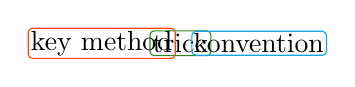
\begin{tikzpicture}
			\node [inner sep=1pt, rounded corners=1.5, draw=ForestGreen] (trick node) {trick};
			\node [inner sep=1pt, rounded corners=1.5, draw=OrangeRed, left of = trick node] {key method};
			\node [inner sep=1pt, rounded corners=1.5, draw=Cerulean, right of = trick node] (convention) {convention};
		\end{tikzpicture}
	}
	\blfootnote{\href{http://arxiv.org/abs/2312.06741}{(CVPR Highlight, 2024) MonoGS: Gaussian Splatting SLAM}}
\end{Frame}

\begin{Frame}{Mapping: Bundle Adjustment \& Random Recall}
	\begin{block}<+->{\alert<.|handout:0>{Bundle Adjustment}}
		\begin{figure}[htbp]
			\centering
			\resetcolorseries[1]{marknode-color-series}
			\resetcolorseries[1]{annotation-color-series}
			\begin{equation}
				\underset{\mathcal{G}, \{\mathbf{T}_{cw}({\mathcal{F}_k})\vert \mathcal{F}_k\in \mathcal{W}\}}{\operatorname{argmin}} \sum_{\mathcal{F}_k}^{\tikzmarknode{n0}{\colorbox{marknode-color-series!![0]}{\scriptsize\(\mathcal{W}\)}}} \mathcal{L}_{pho}\left({\mathcal{F}_k}\right)
			\end{equation}
			\begin{annotatedEquationEnv}
				\annotatedEquation{colorseries}{n0}{north}{0em}{+0.5em}{south west}{annotation-color-series}{keyframes in the sliding window}{east}
			\end{annotatedEquationEnv}
		\end{figure}
		\vspace*{-1.5ex}
	\end{block}
	\vspace*{\fill}
	\begin{block}<+->{\alert<.|handout:0>{Random Recall} \hfill A trick for global mapping}
		\vspace*{0.5ex}
		\par Besides \(\mathcal{W}\), ``some'' randomly selected past keyframes are also leveraged in BA to avoid forgetting the global map.
	\end{block}
	\blfootnote{\href{http://arxiv.org/abs/2312.06741}{(CVPR Highlight, 2024) MonoGS: Gaussian Splatting SLAM}}
\end{Frame}

\begin{Frame}{Mapping: Isotropic Regularization}
	\begin{itemize}
		\setlength{\itemsep}{1.5ex}
		\item<+-> \alert<.>{Why} do we need ``isotropic regularization''?
			\vspace*{1.5ex}
			\begin{itemize}
				\setlength{\itemsep}{1.5ex}
				\item<+-> \alert<.|handout:0>{Observation:} isotropic Gaussians behave better than anisotrophic.
				\item<+-> \alert<.|handout:0>{Analysis:} no constraints on the elongation along the viewing ray direction, \textbf{even with depth}.
			\end{itemize}
	\end{itemize}
	\vspace*{\fill}
	\begin{block}<+->{\alert<.|handout:0>{Isotropic Regularization}}
		\vspace*{0.5ex}
		\begin{equation}
			\mathcal{L}_{iso} = \sum_{i=1}^{\vert \mathcal{G} \vert} \Vert \mathbf{s}_i - \bar{\mathbf{s}}_i \Vert_1, \quad\text{where } \bar{\mathbf{s}}_i = \frac{1}{3} \left( s_i^{x} + s_i^{y} + s_i^{z} \right).
		\end{equation}
	\end{block}
	\blfootnote{\href{http://arxiv.org/abs/2312.06741}{(CVPR Highlight, 2024) MonoGS: Gaussian Splatting SLAM}}
\end{Frame}

\begin{Frame}{Mapping: Conclusion}
	\begin{block}{The Overall Optimization for Mapping}
		\begin{equation}
			\underset{\mathcal{G}, \{\mathbf{T}_{cw}({\mathcal{F}_k})\vert \mathcal{F}_k\in \mathcal{W}^{+}\}}{\operatorname{argmin}} \sum_{\mathcal{F}_k}^{\mathcal{W}^{+}} \mathcal{L}_{pho}\left({\mathcal{F}_k}\right) + \lambda_{iso} \mathcal{L}_{iso}
		\end{equation}
	\end{block}
	\blfootnote{\href{http://arxiv.org/abs/2312.06741}{(CVPR Highlight, 2024) MonoGS: Gaussian Splatting SLAM}}
\end{Frame}

\mode<article>{\section{RTG-SLAM}} \mode<presentation>{\subsection{RTG-SLAM}}

\mode<article>{\subsection{Overview}}
\begin{frame}\mode<presentation>{\Frametitle{Overview}}
	\mode<presentation>{\blfootnote{\href{http://arxiv.org/abs/2404.19706}{(SIGGRAPH 2024) RTG-SLAM: Real-time 3D Reconstruction at Scale using Gaussian Splatting}}}
	\begin{figure}[htbp]
		\centering
		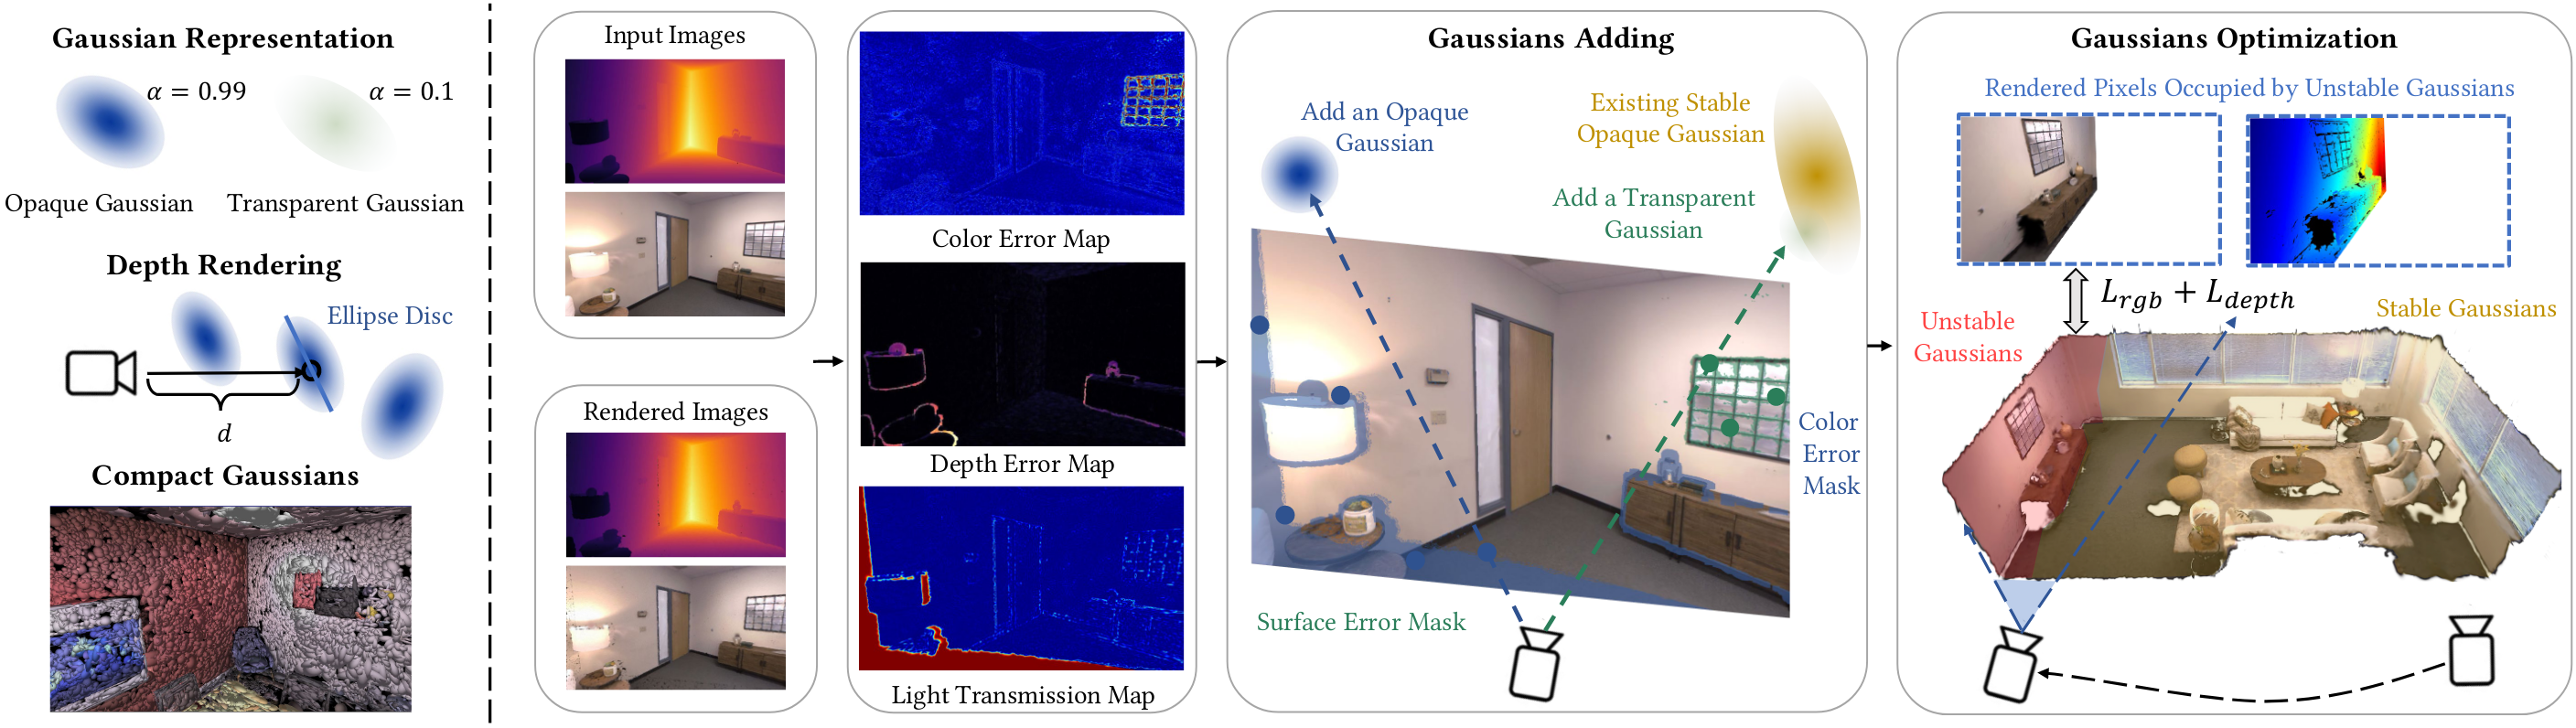
\includegraphics[width=\linewidth]{rtg-slam-overview.png}
		\caption{Overview of RTG-SLAM}
		\label{fig:rtg-slam-overview}
	\end{figure}
\end{frame}

\mode<article>{\subsection{Compact Gaussian Representation}}
\begin{frame}\mode<presentation>{\Frametitle{Compact Gaussian Representation \romannum{1}}}
	\mode<presentation>{\blfootnote{\href{http://arxiv.org/abs/2404.19706}{(SIGGRAPH 2024) RTG-SLAM: Real-time 3D Reconstruction at Scale using Gaussian Splatting}}}
	\mode<article>{
		\par The \alert{compact} 3D Gaussian-based scene representation in RTG-SLAM~\autocite{peng_rtg-slam_2024} can be denoted by equation~\ref{eq:rtg-slam-compact-gaussian}, where the colorful annotations are different from the original 3D Gaussian representation~\autocite{kerbl3Dgaussians}.
	}
	\begin{block}{Compact Gaussian Representation}
		\resetcolorseries[5]{marknode-color-series}
		\resetcolorseries[5]{annotation-color-series}
		\colorlet{marknode-convention}{Gray!20}
		\colorlet{annotation-convention}{Gray}
		\vspace*{1.5em}
		\begin{equation}
			\label{eq:rtg-slam-compact-gaussian}
			\tikzmarknode{n-convention-0}{\colorbox{marknode-convention}{\(\mathcal{S}\)}}  = \left\{ \mathcal{G}_i \vert i = 0,1,\cdots,N \right\}
			,\text{ where }
			\mathcal{G}_i = \left\{
			\tikzmarknode{n-convention-1}{\colorbox{marknode-convention}{\(\mathbf{x}\)}},
			\tikzmarknode{n-convention-2}{\colorbox{marknode-convention}{\(\mathbf{q}\)}},
			\tikzmarknode{n-convention-3}{\colorbox{marknode-convention}{\(\mathbf{s}\)}},
			\tikzmarknode{n-convention-4}{\colorbox{marknode-convention}{\(\mathbf{c}\)}},
			\tikzmarknode{n0}{\colorbox{marknode-color-series!![0]}{\(\alpha\)}},
			\tikzmarknode{n1}{\colorbox{marknode-color-series!![1]}{\(\mathbf{n}\)}},
			\tikzmarknode{n2}{\colorbox{marknode-color-series!![2]}{\(\eta\)}},
			\tikzmarknode{n3}{\colorbox{marknode-color-series!![3]}{\(t\)}}
			\right\}
		\end{equation}
		\begin{annotatedEquationEnv}
			\annotatedEquation{color}{n-convention-0}{north}{0em}{1.5em}{south west}{annotation-convention}{scene}{east}
			\annotatedEquation{color}{n-convention-1}{south}{0em}{-1em}{north east}{annotation-convention}{\(\in \mathbb{R}^3\), position}{west}
			\annotatedEquation{color}{n-convention-2}{south}{0em}{-2.5em}{north east}{annotation-convention}{\(\in \mathrm{SO}(3)\), rotation}{west}
			\annotatedEquation{color}{n-convention-3}{south}{0em}{-4em}{north east}{annotation-convention}{\(\in \mathbb{R}^3\), scale}{west}
			\annotatedEquation{color}{n-convention-4}{south}{0em}{-5.5em}{north east}{annotation-convention}{\(\in \mathbb{R}^{3n}\), color}{west}
			\annotatedEquation{colorseries}{n0}{south}{0em}{-7em}{north east}{annotation-color-series}{\(0.99\vee0.1\), ``boolean'' opacity}{west}
			\annotatedEquation{colorseries}{n1}{south}{0em}{-8.5em}{north east}{annotation-color-series}{\(\in \mathbb{R}^3\), normal vector}{west}
			\annotatedEquation{colorseries}{n2}{south}{0em}{-10em}{north east}{annotation-color-series}{confidence}{west}
			\annotatedEquation{colorseries}{n3}{south}{0em}{-11.5em}{north east}{annotation-color-series}{\(\in \mathbb{R}\), initialization timestamp}{west}
		\end{annotatedEquationEnv}
		\vspace*{11.5em}
	\end{block}
\end{frame}

\begin{frame}\mode<presentation>{\Frametitle{A Review of 3D Gaussian Splattings \romannum{1}}}
	\mode<presentation>{\blfootnote{\href{http://arxiv.org/abs/2404.19706}{(SIGGRAPH 2024) RTG-SLAM: Real-time 3D Reconstruction at Scale using Gaussian Splatting}}}
	\mode<article>{
		\par The appearance (RGB) rendering is basically the same as the original 3DGS. For the current frame, the Gaussians are sorted from front to back and re-indexed from \(0\) to \(N\), and then alpha-blending (equation~\ref{eq:alpha-blending}) is leveraged for image formation.
	}
	\begin{block}{\(\boldsymbol\alpha\)-blending\hfill Image Formation Model}
		\vspace*{6.5em}
		\resetcolorseries[6]{marknode-color-series}
		\resetcolorseries[6]{annotation-color-series}
		\begin{equation}\label{eq:alpha-blending}
			\tikzmarknode{n0}{\colorbox{marknode-color-series!![0]}{\(\hat{\mathbf{C}}\)}}
			(
			\tikzmarknode{n1}{\colorbox{marknode-color-series!![1]}{\(\mathbf{u}\)}}
			)
			=
			\sum_{
				i
				=0}^{
			\tikzmarknode{n2}{\colorbox{marknode-color-series!![2]}{\scriptsize \(N\)}}
			}
			\tikzmarknode{n3}{\colorbox{marknode-color-series!![3]}{\(\mathbf{c}_i\)}}
			\tikzmarknode{n4}{\colorbox{marknode-color-series!![4]}{\(p_i\)}}
			(\mathbf{u})
			\alpha_i
			\tikzmarknode{n5}{\colorbox{marknode-color-series!![5]}{\(\displaystyle \prod_{j=0}^{i-1} (1-p_j(\mathbf{u})\alpha_j)\)}}
		\end{equation}
		\begin{annotatedEquationEnv}
			\annotatedEquation{colorseries}{n0}{north}{0em}{6.5em}{south west}{annotation-color-series}{\(\mathbb{R}^{2} \mapsto \mathbb{R}^{3}\), the rendered RGB image}{east}
			\annotatedEquation{colorseries}{n1}{north}{0em}{5.5em}{south west}{annotation-color-series}{\(= \begin{bmatrix}
				h & w
			\end{bmatrix}^{\mathrm{T}}\), a pixel}{east}
			\annotatedEquation{colorseries}{n2}{north}{0em}{3em}{south west}{annotation-color-series}{the number of sorted and visible 3D Gaussians}{east}
			\annotatedEquation{colorseries}{n3}{south}{0em}{-4em}{north west}{annotation-color-series}{color of \(i\)-th Gaussian}{east}
			\annotatedEquation{colorseries}{n4}{south}{0em}{-1.5em}{north west}{annotation-color-series}{\(\mathbb{R}^{2} \mapsto [0,1]\), probability distribution of \\ \(i\)-th splatted(2D) Gaussian}{east}
			\annotatedEquation{colorseries}{n5}{north}{0em}{1em}{south west}{annotation-color-series}{\(T_i \in \mathbb{R}\), \\transmittance for \(i\)-th Gaussian}{east}
		\end{annotatedEquationEnv}
		\vspace*{4em}
	\end{block}
\end{frame}

\begin{frame}
	\mode<presentation>{\Frametitle{A Review of 3D Gaussian Splattings \romannum{2}}}
	\mode<presentation>{\blfootnote{\href{http://arxiv.org/abs/2404.19706}{(SIGGRAPH 2024) RTG-SLAM: Real-time 3D Reconstruction at Scale using Gaussian Splatting}}}
\end{frame}



\alt<article>{\chapter*{References}}{\section{References}}
\begin{frame}[allowframebreaks]
	\mode<presentation>{\frametitle{References}}
	% \nocite{*}
	\printbibliography[heading=none]
\end{frame}

\appendix % \section{\appendixname}
\mode<article>{\chapter{Mathematical Prerequistes}}
\mode<article>{\section{Ray-plane Intersection}\label{appendix:ray-plane-intersection}}
\begin{frame}<all>[c]
	\mode<presentation>{\Frametitle{Ray-plane Intersection}}
	\par Let the ray and the plane be given parametrically by equation~\ref{eq:appendix-ray} and equation~\ref{eq:appendix-plane}.
	\par
	\begin{minipage}[t]{0.45\linewidth}
		\resetcolorseries[4]{marknode-color-series}
		\resetcolorseries[4]{annotation-color-series}
		\begin{equation}
			\label{eq:appendix-ray}
			\tikzmarknode{n0}{\colorbox{marknode-color-series!![0]}{\(\mathbf{q}\)}}
			=
			\tikzmarknode{n1}{\colorbox{marknode-color-series!![1]}{\(\mathbf{p}\)}}
			+
			\tikzmarknode{n2}{\colorbox{marknode-color-series!![2]}{\(t\)}}
			\tikzmarknode{n3}{\colorbox{marknode-color-series!![3]}{\(\mathbf{v}\)}}
			,
		\end{equation}
		\vspace*{5em}
		\begin{annotatedEquationEnv}
			\annotatedEquation{colorseries}{n0}{south}{0em}{-0.5em}{north east}{annotation-color-series}{\(\in \mathbb{R}^3\), point on the ray}{west}
			\annotatedEquation{colorseries}{n1}{south}{0em}{-4em}{north west}{annotation-color-series}{\(\in \mathbb{R}^3\), initial point}{east}
			\annotatedEquation{colorseries}{n2}{south}{0em}{-3em}{north west}{annotation-color-series}{\(\in \mathbb{R}, t \geq 0\), length}{east}
			\annotatedEquation{colorseries}{n3}{south}{0em}{-0.5em}{north west}{annotation-color-series}{\(\in \mathbb{R}^3, \Vert \mathbf{v} \Vert = 1\), \\direction vector}{east}
		\end{annotatedEquationEnv}
	\end{minipage}
	\begin{minipage}[t]{0.45\linewidth}
		\resetcolorseries[3]{marknode-color-series}
		\resetcolorseries[3]{annotation-color-series}
		\begin{equation}
			\label{eq:appendix-plane}
			\langle
			\tikzmarknode{n0}{\colorbox{marknode-color-series!![0]}{\(\mathbf{n}\)}}
			,
			\tikzmarknode{n1}{\colorbox{marknode-color-series!![1]}{\(\mathbf{r}\)}}
			\rangle
			+
			\tikzmarknode{n2}{\colorbox{marknode-color-series!![2]}{\(d\)}}
			= 0.
		\end{equation}
		\begin{annotatedEquationEnv}
			\annotatedEquation{colorseries}{n0}{south}{0em}{-3.5em}{north west}{annotation-color-series}{\(\in \mathbb{R}^3\), normal vector}{east}
			\annotatedEquation{colorseries}{n1}{south}{0em}{-2em}{north west}{annotation-color-series}{\(\in \mathbb{R}^3\), point on the plane}{east}
			\annotatedEquation{colorseries}{n2}{south}{0em}{-0.5em}{north west}{annotation-color-series}{\(\in \mathbb{R}\), translation}{east}
		\end{annotatedEquationEnv}
	\end{minipage}
	\par\noindent The ray-plane intersection occurs when \(\mathbf{q}\) satisfies the plane equation. Substituting and rearranging, we can acquire the length from the initial point of the ray and the intersection,
	\begin{align}
		% \label{eq:}
		0 & = \langle \mathbf{n}, \left( \mathbf{p} + t \mathbf{v} \right) \rangle + d                    \\
		0 & = \langle \mathbf{n}, \mathbf{p} \rangle + t \langle \mathbf{n},\mathbf{v} \rangle + d        \\
		t & = -\frac{d + \langle \mathbf{n}, \mathbf{p} \rangle}{\langle \mathbf{n}, \mathbf{v} \rangle}.
	\end{align}
\end{frame}

\mode<article>{\chapter{Traditional SLAM}}
\mode<article>{\section{KinectFusion}}
\begin{frame}<all>[c]
	\mode<presentation>{\Frametitle{KinectFusion}}
\end{frame}

\mode<article>{\backmatter}

\end{document}
